\chapter{Booting a PC}
\label{cha:booting_a_pc}

%TODO: 环境搭建

\section{PC Bootstrap}
\par 这一部分主要介绍了x86语言以及PC的启动过程,并让我们熟悉了QEMU和GDB的调试方法。

\subsection{Getting Started with x86 assembly}
\par 通过阅读\emph{PC Assembly Language Book}\footnote{\url{https://pdos.csail.mit.edu/6.828/2017/readings/pcasm-book.pdf}}来学习x86的语法。注意这本书值使用的NASM汇编,但是实验中使用的是GNU的AT\&T语法。

\exercise{1}{
    \par 了解和学习x86的语法。
}

\begin{exerciseSolution}{1}
\par 由于已经上过intel汇编的理论课,因此这一部大部分为复习内容。通过阅读所给的参考文献,并结合以往的经验来看,较为重要的部分是熟悉汇编的语法,各个指令的作用以及能够掌握C语言与汇编的关系。
\end{exerciseSolution}

\subsection{Simulating the x86}
\par 首先安装qemu虚拟机以及计算所使用的工具链,以及调试工具GDB。此次实验使用的为Arch Linux,且在实验过程中发现gcc7.3.0不能够正确的对jos源码进行编译,因此所使用的的gcc为从源码编译的i386-jos-elf-gcc。QEMU则是使用的Arch Linux官方源中的qemu。
\par 在安装完成后,进入目录并使用make进行编译。编译完成后使用make qemu命令启动qemu。启动后的QEMU如图\ref{fig:exercise1_1}所示。
\begin{figure}[htb]
    \centering
    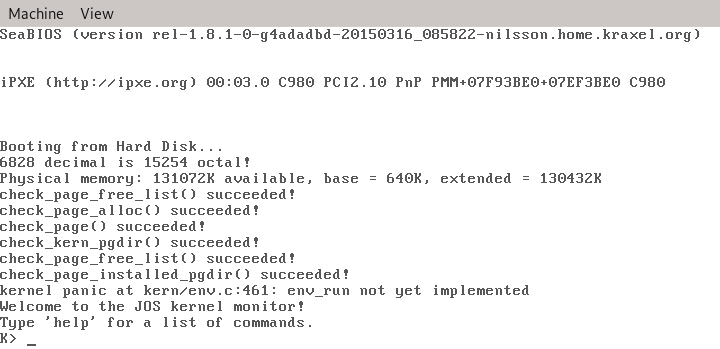
\includegraphics[width=0.8\linewidth]{lab1/exercise1_1.png}
    \caption{初次编译成功并启动的qemu}
    \label{fig:exercise1_1}
\end{figure}

\par 可以发jos内核已经正常启动,并且能够执行help命令。执行help命令以后显示最初始的jOS由两个命令:help以及kerninfo。输入kerninfo命令以后命令行中打印出了部分有关内核的信息。

\FloatBarrier
\subsection{The PC's Physical Address Space}
\par 从实验指导中可以知道,通常情况下一个PC的布局是如图\ref{fig:exercise1_3}所示的。
\begin{figure}[htb]
    \centering
    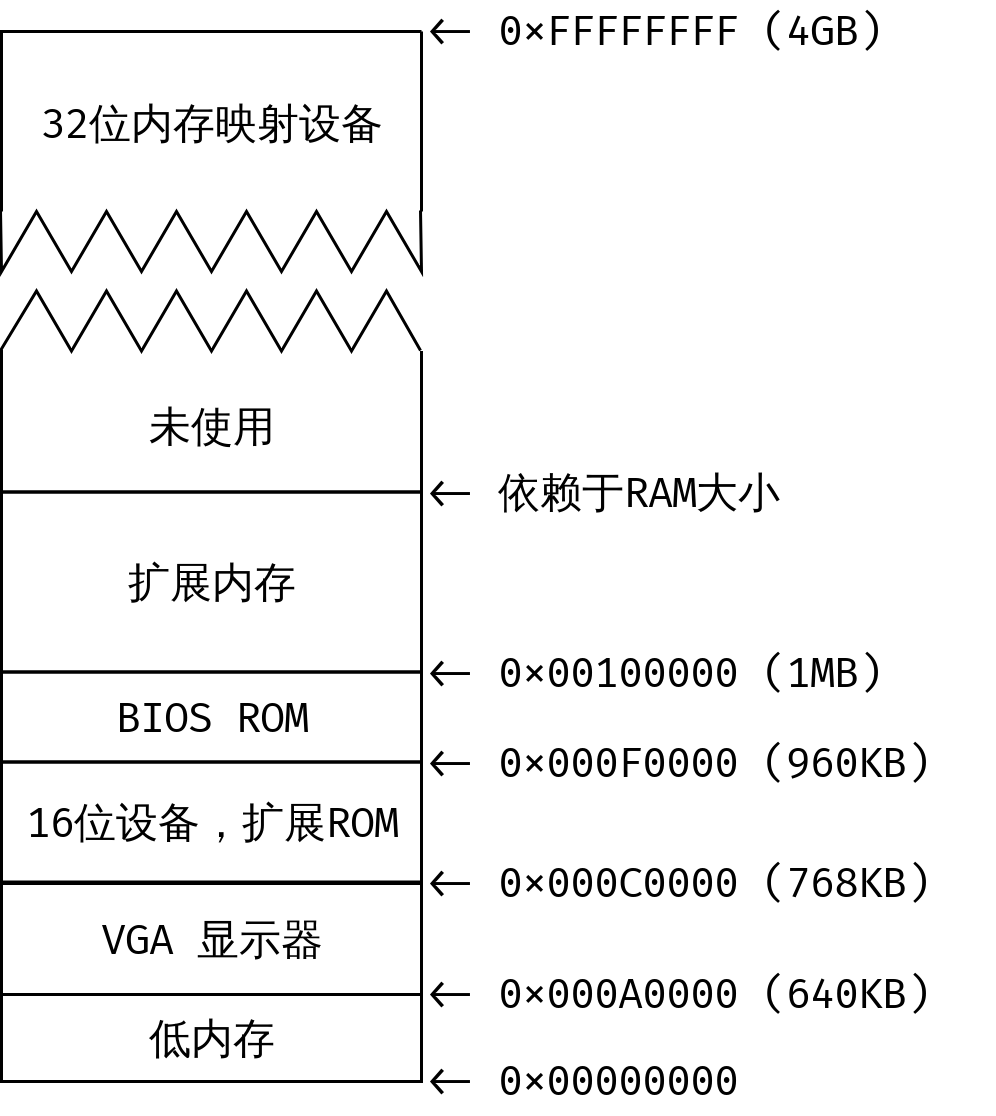
\includegraphics[width=0.38\linewidth]{lab1/exercise1_3.png}
    \caption{内存布局}
    \label{fig:exercise1_3}
\end{figure}

\par 在早期的16位8088处理器只能够操作1MB物理内存,因此物理地址空间为0x00000000到0x000FFFFF。其中0\textasciitilde 640KB为Low Memory,只能被RAM所使用。而从0x000A0000到0x000FFFFF的384KB内存保留做特殊用途,包括显示缓存以及其他固件。从0x000F0000到0x000FFFFF这64KB区域为BIOS。现代x86处理器支持4GB的RAM,因此RAM扩展到了0xFFFFFFFF,但jos只使用开始的256MB。

\FloatBarrier
\subsection{The ROM BIOS}
\par 在一个终端下执行make qemu-gdb指令,然后新建一个terminal,执行make gdb指令,结果如图\ref{fig:exercise1_4}所示(此处使用的是cgb,便于调试,此后的调试也将使用cgdb而不是gdb)。可以看到,gdb已经开始调试并停止在0xffff0处。而这条指令就是PC启动后BIOS执行的第一条指令。
\begin{figure}[htb]
    \centering
    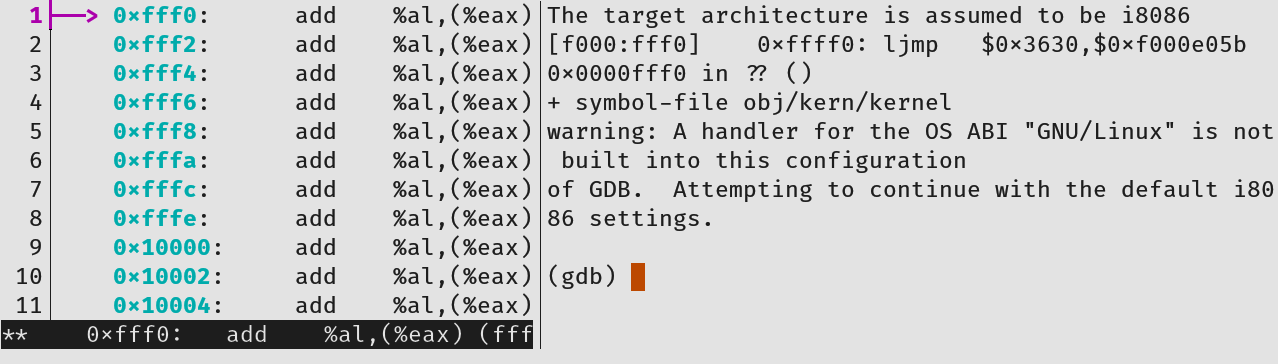
\includegraphics[width=0.9\linewidth]{lab1/exercise1_4.png}
    \caption{初次进入调试界面}
    \label{fig:exercise1_4}
\end{figure}

\par 第一条指令表明:
\begin{itemize}
    \item IBM PC 执行的起始物理地址为 0x000ffff0
    \item PC 的偏移方式为 CS = 0xf000,IP = 0xfff0
    \item 第一条指令执行的是 jmp指令,跳转到段地址 CS = 0xf000,IP = 0xe05b
\end{itemize}

\exercise{2}{
    \par 使用GDB的si命令单步调试进入ROM BIOS,然后猜测这些指令的作用。
}

\begin{exerciseSolution}{2}
\par 在使用make qemu-gdb命令编译内核并启动qemu,然后使用make gdb命令启动gdb后,使用si单步调试。连续执行si命令多步后,得到的前30条指令如下:

\inputCodeSetLanguage{[x86masm]Assembler}
\begin{lstlisting}
0xffff0:  ljmp   $0xf000, $0xe05b
0xfe05b:  cmpl   $0x0,    $cs:0x6ac8
0xfe062:  jne    0xfd2e1
0xfe066:  xor    %dx,     %dx
0xfe068:  mov    %dx,     %ss
0xfe06a:  mov    $0x7000, %esp
0xfe070:  mov    $0xf34d2,%edx
0xfe076:  jmp    0xfd15c
0xfd15c:  mov    %eax,    %ecx
0xfd15f:  cli
0xfd160:  cld
0xfd161:  mov    $0x8f,   %eax
0xfd167:  out    %al,     $0x70
0xfd169:  in     $0x71,   %al
0xfd16b:  in     $0x92,   %al
0xfd16d:  or     $0x2,    %al
0xfd16f:  out    %al,     $0x92
0xfd171:  lidtw  %cs:0x6ab8
0xfd177:  lgdtw  %cs:0x6a74
0xfd17d:  mov    %cr0,    %eax
0xfd180:  or     $0x1,    %eax
0xfd184:  mov    %eax,    %cr0
0xfd187:  ljmpl  $0x8,    $0xfd18f
0xfd18f:  mov    $0x10,   %eax
0xfd194:  mov    %eax,    %ds
0xfd196:  mov    %eax,    %es
0xfd198:  mov    %eax,    %ss
0xfd19a:  mov    %eax,    %fs
0xfd19c:  mov    %eax,    %gs
0xfd19e:  mov    %ecx,    %eax
\end{lstlisting}

其中:
\begin{itemize}
    \item 第1条指令是一条跳转指令,跳转到0xfe05b处。
    \item 第2条和第3条指令共同构成了判断跳转,如果\$cs:0x6ac8处的值不为0则跳转,而根据第4条指令的地址可以得知此处并没有发生跳转。
    \item 第4跳指令将\%dx清零。
    \item 第5\textasciitilde 8条指令在设置完段寄存器、段指针以及edx寄存器后跳转到了0xfd15c处。然后第10跳指令关闭了中断。这应该是由于boot过程是比较关键的,因此屏蔽大部分的中断。
    \item 第11跳指令设置了方向标志位,表示后续操作的内存变化方向。
    \item 第12\textasciitilde 14条指令涉及到IO操作。CPU与外部设备通讯需要通过IO端口访问,而x86CPU使用IO端口独立编址的方式。并且规定端口操作需要通过al或者ax进行。通过查询端口对应的设备\footnote{\url{http://bochs.sourceforge.net/techspec/PORTS.LST}}我们知道了0x70和0x71是用于操作CMOS的端口。而这三条指令是用于关闭不可屏蔽中断(Non-Maskable Interrupt)的。
    \item 第18和19条指令用于将0xf6ab8处的数据读入到中断向量表寄存器(IDTR)中,并将0xf6a74的数据读入到全局描述符表格寄存器(GDTR)中,而后者是实现保护模式中较为重要的一部分。
    \item 第20\textasciitilde 21用于将CR0寄存器的最低位置1,进入保护模式,然而后面又从保护模式退出,继续在实模式下运行。
    \item 第23\textasciitilde 29步用于重新加载段寄存器,在加载完GDTR寄存器后需要刷新所有的段寄存器的值\footnote{\url{https://en.wikibooks.org/wiki/X86_Assembly/Global_Descriptor_Table}} 。
\end{itemize}
\end{exerciseSolution}

\section{The Bootloader}
\par 对于PC而言软盘和硬盘都被分为512字节的扇区。一个扇区是磁盘传输的最小粒度,也就是说读写都必须以扇区为单位执行。如果一个磁盘是可启动的,就把这个磁盘的第一个扇区叫做启动扇区,而boot loader就位于这一个扇区中。当BIOS找到一个可以启动的磁盘以后就会把这512字节的扇区加载到0x7c00到0x7dff中。

\par jOS采用传统的硬盘启动机制,也就是说boot loader的大小小于512字节。bootloader只包含两个文件:一个汇编文件boot/boot.S和一个C文件boot/main.c,并且主要有如下两个功能:
\begin{itemize}
    \item 将处理器由实模式转换为保护模式。
    \item 通过x86的特殊I/O访问指令将内核从硬盘读入内存。
\end{itemize}

\exercise{3}{
    \par 在0x7c00处设置断点,然后让程序运行到这个断点,然后使用gdb跟踪boot.S的每一条指令,并比较obj/boot/boot.asm以及boot/boot.S。
    \par 追踪进入bootmain()中,然后追踪进入readsect()中,并找出每一条readsect()中c语句对应的汇编语句,然后找出把内核从磁盘读取到内存的for语句对应的汇编语句。找出loop运行完后那些语句会被执行,并在那里设置断点。继续运行到断点然后执行完接下来的语句。
}

\begin{exerciseSolution}{3}
\par 首先使用make qemu-gdb命令启动qemu,然后使用make gdb命令启动gdb并在gdb中使用b *0x7c00打上断点,然后使用c命令执行到此断点处。
\par 从反汇编的代码obj/boot/boot.asm中可以看出,0x7c00就是boot loader的起始地址。也就是说,实验要求我们从boot loader的开始处跟踪。

\par 首先观察并分析boot.S以及main.c中的内容,分析每一个部分的作用,以便于后续的跟踪:
\inputCodeSetLanguage{[x86masm]Assembler}
\begin{lstlisting}
.globl start
start:
  .code16                     # Assemble for 16-bit mode
  cli                         # Disable interrupts
  cld                         # String operations increment
  # Set up the important data segment registers (DS, ES, SS).
  xorw    %ax,%ax             # Segment number zero
  movw    %ax,%ds             # -> Data Segment
  movw    %ax,%es             # -> Extra Segment
  movw    %ax,%ss             # -> Stack Segment
\end{lstlisting}
\par 在boot.S的开始部分,首先关闭了在BIOS运行期间可能打开的中断,防止boot loader在运行期间被中断。cld用于设置字符串处理时指针的移动方向。
\par 从xorw开始的4句代码用于将段寄存器清零:首先将寄存器\%ax置为0,然后将\%ax赋值给段寄存器\%ds, \%es, \%ss。由于在BIOS阶段这些寄存器的值可能发生改变因此此处需要对其进行复位操作。

\par 在上述准备代码完成后,执行从实模式到保护模式的代码:
\begin{lstlisting}
  # Enable A20:
  #   For backwards compatibility with the earliest PCs, physical
  #   address line 20 is tied low, so that addresses higher than
  #   1MB wrap around to zero by default.  This code undoes this.
seta20.1:
  inb     $0x64,%al               # Wait for not busy
  testb   $0x2,%al
  jnz     seta20.1

  movb    $0xd1,%al               # 0xd1 -> port 0x64
  outb    %al,$0x64

seta20.2:
  inb     $0x64,%al               # Wait for not busy
  testb   $0x2,%al
  jnz     seta20.2

  movb    $0xdf,%al               # 0xdf -> port 0x60
  outb    %al,$0x60
\end{lstlisting}
\par 这部分代码用于将CPU从实模式转换为保护模式:为了保留对于早期计算机的后向兼容性,第20根物理地址线保持为0,因此所有大于1MB的地址全部会回卷,而这段代码解除了这一限制。
\par seta20.1后面的3句指令不停地检测0x64端口的第0x2位,若其不为0则重复这一检测。这三句命令用于阻塞直到输入缓冲区为空。当缓冲区准备完成后,movb和outb指令向0x64端口写入0xd1。经过查询,0xd1指令的作用是将下一次写入0x60端口的指令会被发送给键盘控制器804x的输入端口。
\par seta20.2后面的三句与seta20.1后面的三句相同,再次等待缓冲区可以切入。在等待完成后的movb和outb指令向0x60端口写入数据0xdf。0xdf表示使能A20线,可以进入保护模式。

\begin{lstlisting}
  # Switch from real to protected mode, using a bootstrap GDT
  # and segment translation that makes virtual addresses
  # identical to their physical addresses, so that the
  # effective memory map does not change during the switch.
  lgdt    gdtdesc
  movl    %cr0, %eax
  orl     $CR0_PE_ON, %eax
  movl    %eax, %cr0

  # Jump to next instruction, but in 32-bit code segment.
  # Switches processor into 32-bit mode.
  ljmp    $PROT_MODE_CSEG, $protcseg
\end{lstlisting}

\par 使能A20线后,首先把gdtdesc标识符送入GDTR中。GDTR有48位长,其中高32位表示该表在内存中的起始地址,低16位表示该表的长度。这一指令就是将GDT表的起始地址以及长度送入GDTR中。gdtdsec的标识符内容在boot.S尾部:
\begin{lstlisting}
gdtdesc:
  .word   0x17                            # sizeof(gdt) - 1
  .long   gdt                             # address gdt
\end{lstlisting}
\par 可以看出gdt表的大小为0x17,表的起始地址为标号gdt所在的位置。
\par 在加载完GDT表的信息到GDTR后,使用了三个指令修改给\%cr0寄存器的内容。从文件首可以找到:
\begin{lstlisting}
.set PROT_MODE_CSEG, 0x8         # kernel code segment selector
.set PROT_MODE_DSEG, 0x10        # kernel data segment selector
.set CR0_PE_ON,      0x1         # protected mode enable flag
\end{lstlisting}

\par 也就是说,这几句将寄存器\%cr0的最低位置为1,而\%cr0的最低位是保护模式的启动位,将CR0的这一位置为1则表示保护模式启动。
\par 在正式启动保护模式后,执行了一个ljmp指令,将当前的运行模式切换为32为地址模式。接下来运行的就是32位的代码:

\begin{lstlisting}
  .code32                     # Assemble for 32-bit mode
protcseg:
  # Set up the protected-mode data segment registers
  movw    $PROT_MODE_DSEG, %ax    # Our data segment selector
  movw    %ax, %ds                # -> DS: Data Segment
  movw    %ax, %es                # -> ES: Extra Segment
  movw    %ax, %fs                # -> FS
  movw    %ax, %gs                # -> GS
  movw    %ax, %ss                # -> SS: Stack Segment

  # Set up the stack pointer and call into C.
  movl    $start, %esp
  call bootmain
\end{lstlisting}
\par 在32位的代码开头,修改了5个段寄存器的值。与前述BIOS部分一样,当加载完GDTR后必须重新加载段寄存器的值,而加载CS的值必须通过ljmp加载(也就是将运行模式切换为32位地址模式的指令)。从而使GDTR生效。然后设置完栈指针的值后,跳转到bootmain中去。

\par 在main.c中,bootmain函数如下:
\inputCodeSetLanguage{c}
\begin{lstlisting}
void
bootmain(void)
{
    struct Proghdr *ph, *eph;

    // read 1st page off disk
    readseg((uint32_t) ELFHDR, SECTSIZE*8, 0);

    // is this a valid ELF?
    if (ELFHDR->e_magic != ELF_MAGIC)
        goto bad;

    // load each program segment (ignores ph flags)
    ph = (struct Proghdr *) ((uint8_t *) ELFHDR + ELFHDR->e_phoff);
    eph = ph + ELFHDR->e_phnum;
    for (; ph < eph; ph++)
        // p_pa is the load address of this segment (as well
        // as the physical address)
        readseg(ph->p_pa, ph->p_memsz, ph->p_offset);

    // call the entry point from the ELF header
    // note: does not return!
    ((void (*)(void)) (ELFHDR->e_entry))();

bad:
    outw(0x8A00, 0x8A00);
    outw(0x8A00, 0x8E00);
    while (1)
        /* do nothing */;
}
\end{lstlisting}

\par 从代码中可以看出,首先bootmain调用了readseg函数:
\begin{lstlisting}
// Read 'count' bytes at 'offset' from kernel into physical address 'pa'.
// Might copy more than asked
void
readseg(uint32_t pa, uint32_t count, uint32_t offset)
\end{lstlisting}

\par 而从readseg函数定义处的注释可以看出,这个函数的作用是:将从offset开始的count个字节读到pa所在的位置。因此在bootmain中,readseg((uint32\_t) ELFHDR, SECTSIZE*8, 0);这条语句的作用是将内核的第一页($SECTSIZE\times 8 = 4096$)的内容读取到ELFHDR处,也就是说,把内核的elf头部放入内存开始部分。
\par 然后,下一条语句验证这是否是一个合法的elf文件头部。如果不是则跳转到bad标签处。
\par 然后,在elf头部找到程序的段信息。而e\_phoff表示的是ProgramHeaderTable距离elf起始地址的偏移量。将这一偏移量加上elf的起始地址存入ph中,作为ProgramHeaderTable的起始地址,然后通过偏移量将eph作为其结束地址。
\par 接下来的for循环就是加载所有的段进入内存中。p\_offset值得是这一段开头相对于elf文件开头的偏移量,ph\_memsz指的是这个段被装入内存后的大小,而p\_pa指的则是装入内存的起始地址。
\par 最后((void (*)(void)) (ELFHDR->e\_entry))();语句执行e\_entry。e\_entry是执行的入口地址,也就是说,通过执行这个地址的方式把控制权从bootloader转移给内核。

\begin{figure}[htb]
    \centering
    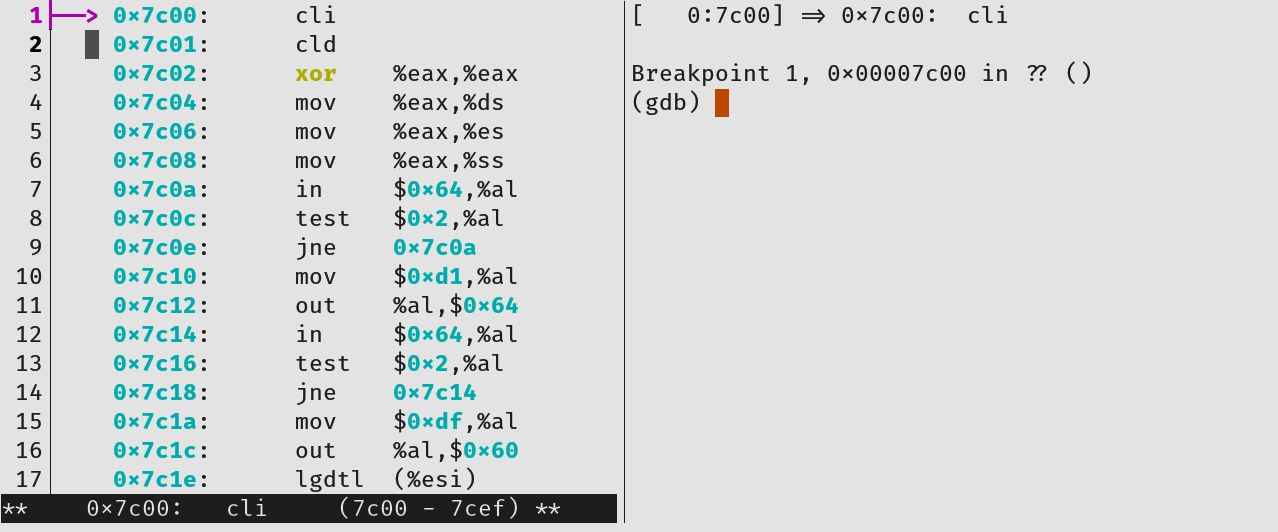
\includegraphics[width=0.9\linewidth]{lab1/exercise3_1.png}
    \caption{gdb反汇编代码}
    \label{fig:exercise3_1}
\end{figure}
\par 接下来,开始使用gdb进行跟踪。首先设置断点,然后运行到断点处。gdb反汇编代码如\ref{fig:exercise3_1}所示,图中显示了GDB反汇编的起始17条指令

\FloatBarrier
\par 下面为boot/boot.S的前17条指令
\inputCodeSetLanguage{[x86masm]Assembler}
\begin{lstlisting}
.set PROT_MODE_CSEG, 0x8         # kernel code segment selector
.set PROT_MODE_DSEG, 0x10        # kernel data segment selector
.set CR0_PE_ON,      0x1         # protected mode enable flag

.globl start
start:
  .code16                     # Assemble for 16-bit mode
  cli                         # Disable interrupts
  cld                         # String operations increment

  # Set up the important data segment registers (DS, ES, SS).
  xorw    %ax,%ax             # Segment number zero
  movw    %ax,%ds             # -> Data Segment
  movw    %ax,%es             # -> Extra Segment
  movw    %ax,%ss             # -> Stack Segment

  # Enable A20:
  #   For backwards compatibility with the earliest PCs, physical
  #   address line 20 is tied low, so that addresses higher than
  #   1MB wrap around to zero by default.  This code undoes this.
seta20.1:
  inb     $0x64,%al               # Wait for not busy
  testb   $0x2,%al
  jnz     seta20.1

  movb    $0xd1,%al               # 0xd1 -> port 0x64
\end{lstlisting}

\par 然后是obj/boot/boot.asm中的前10条指令:
\begin{lstlisting}
.globl start
start:
  .code16                     # Assemble for 16-bit mode
  cli                         # Disable interrupts
    7c00:	fa                   	cli
  cld                         # String operations increment
    7c01:	fc                   	cld

  # Set up the important data segment registers (DS, ES, SS).
  xorw    %ax,%ax             # Segment number zero
    7c02:	31 c0                	xor    %eax,%eax
  movw    %ax,%ds             # -> Data Segment
    7c04:	8e d8                	mov    %eax,%ds
  movw    %ax,%es             # -> Extra Segment
    7c06:	8e c0                	mov    %eax,%es
  movw    %ax,%ss             # -> Stack Segment
    7c08:	8e d0                	mov    %eax,%ss

00007c0a <seta20.1>:
  # Enable A20:
  #   For backwards compatibility with the earliest PCs, physical
  #   address line 20 is tied low, so that addresses higher than
  #   1MB wrap around to zero by default.  This code undoes this.
seta20.1:
  inb     $0x64,%al               # Wait for not busy
    7c0a:	e4 64                	in     $0x64,%al
  testb   $0x2,%al
    7c0c:	a8 02                	test   $0x2,%al
  jnz     seta20.1
    7c0e:	75 fa                	jne    7c0a <seta20.1>

  movb    $0xd1,%al               # 0xd1 -> port 0x64
    7c10:	b0 d1                	mov    $0xd1,%al
\end{lstlisting}
\par 通过比较可以发现,源程序中如movb,inb等指令在gdb中实际执行的是mov,in指令,用于标识操作数长度的后缀没有了,但是指令的实际功能是相同的。在boot/boot.S中的标识在gdb中变为了实际的物理地址。而在boot.asm中则同时包含了这两项,即转换前使用标识标示地址以及编译后使用真实地址表示地址的。此外boot/boot.S中的注释是不被编译的。

\begin{figure}[htb]
    \centering
    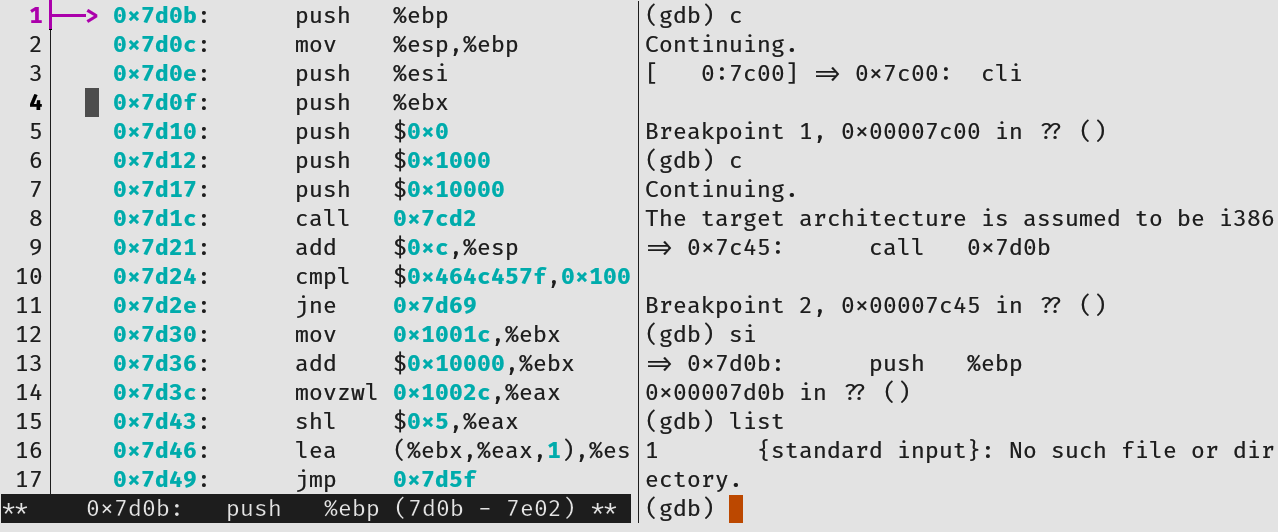
\includegraphics[width=0.9\linewidth]{lab1/exercise3_2.png}
    \caption{gdb中bootmain的反汇编}
    \label{fig:exercise3_2}
\end{figure}
\par 继续执行,一直执行到call bootmain处。执行完后gdb反汇编如\ref{fig:exercise3_2}所示。

\par bootmain中,7d0b到7d0f处的4条语句是C语言执行函数调用的时候必须要进行的一些任务,包括修改栈帧信息以及保护寄存器\%esi,\%ebx的值。在进行了这些必要的任务后。7d10到7d12处的指令是对于参数的压栈,以将参数传递给regadseg函数。压栈完成后使用call语句调用readseg函数。

\begin{figure}[htb]
    \centering
    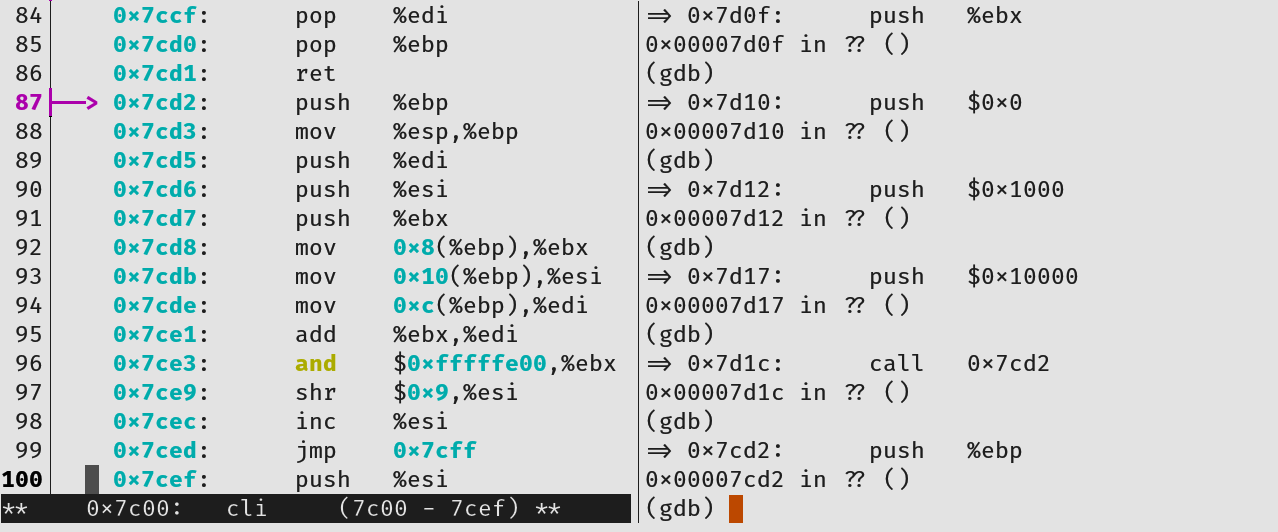
\includegraphics[width=0.9\linewidth]{lab1/exercise3_3.png}
    \caption{gdb中readseg函数的反汇编}
    \label{fig:exercise3_3}
\end{figure}
\par Excercise 3要求追踪到readsect函数中,因此继续向下追踪。执行到readseg函数时,反汇编如图\ref{fig:exercise3_3}所示。

\par 在readseg函数中,7cd2到7cdb处的程序依然是例行执行的修改栈帧、保护寄存器、初始化局部变量等。7cde到7cec处的汇编语句用于计算end\_pa、pa、offset,为后面读取内核做准备。从这三句汇编语言可以看出一句C语言语句可能对应不止一句汇编语句。
\par 在计算完起始地址,结束地址,偏移量后,进入while循环。在进入循环的第一条指令为jmp 7cff,进行了一个绝对跳转。实际上,C语言实现while循环一般是先进行跳转,将判断的语句置于循环体之后,也就是将while实现为do-while的形式。进行判断的语句为:
\begin{lstlisting}
7cff:	39 fb                	cmp    %edi,%ebx
7d01:	72 ec                	jb     7cef <readseg+0x1d>
\end{lstlisting}
\par 在进行了判断后,跳转到7cef,而7cef正是循环体的开始地址。在循环体中,一共执行了3条C语言语句:
\inputCodeSetLanguage{c}
\begin{lstlisting}
readsect((uint8_t*) pa, offset);
pa += SECTSIZE;
offset++;
\end{lstlisting}

\par 从这三条语句中可以看出,readseg是通过调用readsect来逐个扇区将数据读入内存从而达到加载整个段的效果。下面使用gdb继续追踪进入readsect中。此时gdb的反汇编如\ref{fig:exercise3_4}所示。
\begin{figure}[htb]
    \centering
    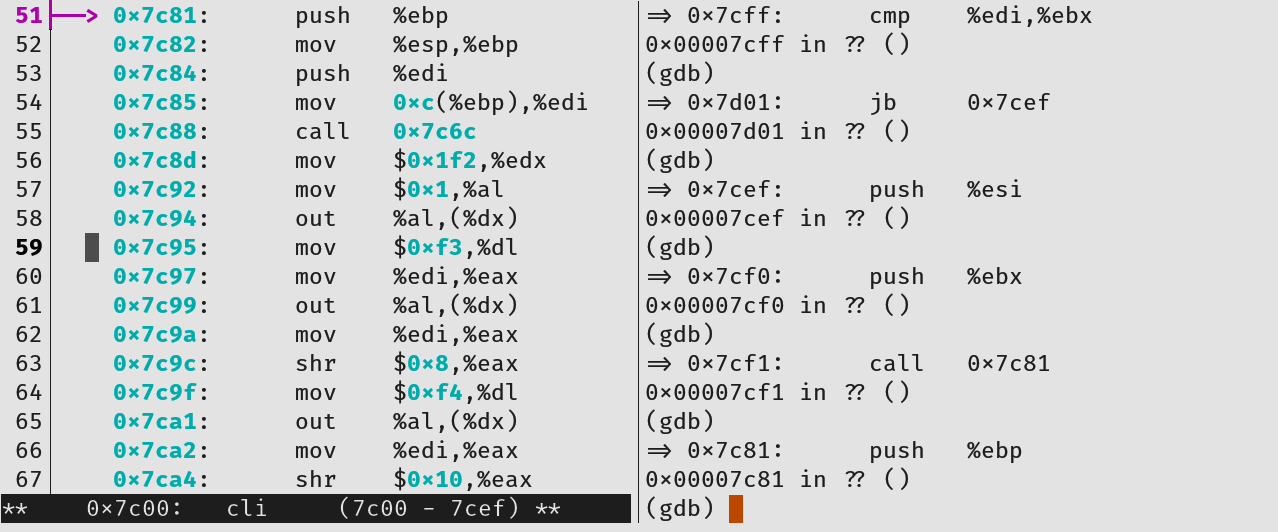
\includegraphics[width=0.9\linewidth]{lab1/exercise3_4.png}
    \caption{readsect在gdb中的反汇编}
    \label{fig:exercise3_4}
\end{figure}

\par 从反汇编中可以看出,readsect函数体执行的第一个语句为waitdisk。而根据注释可以知道这一语句用于等待磁盘空闲。在磁盘空闲后,执行了一系列outb语句,这一系列outb语句用于向端口写值。第一个outb语句对应的汇编为:
\inputCodeSetLanguage{[x86masm]Assembler}
\begin{lstlisting}
7c8d:	ba f2 01 00 00       	mov    $0x1f2,%edx
7c92:	b0 01                	mov    $0x1,%al
7c94:	ee                   	out    %al,(%dx)
\end{lstlisting}

\par 可以看出,C语言中outb的实现就是使用汇编的out语句实现的端口IO。从所有outb语句对应的7c8d到7cb9之间的汇编语句可以看出:outb语句中第一个参数是端口号,第二个参数是送入端口的值。然后经过查询得知,这一函数首先向端口0x1f2送入值1,这表示取出一个扇区;然后将要取出的扇区的32位编号分为4段,分别送入0x1f3到0x1f6,最后向0x1f7端口送入0x20指令,表示要读取这个扇区。
\par 在上述的一系列动作完成后,调用waitdisk()阻塞并等待磁盘读取完成。读取完成后继续执行下一条语句,即insl语句。insl函数对应的汇编指令如下。
\begin{lstlisting}
7cbf:	8b 7d 08             	mov    0x8(%ebp),%edi
7cc2:	b9 80 00 00 00       	mov    $0x80,%ecx
7cc7:	ba f0 01 00 00       	mov    $0x1f0,%edx
7ccc:	fc                   	cld
7ccd:	f2 6d                	repnz insl (%dx),%es:(%edi)
\end{lstlisting}
\par 可以看出,insl函数有3个参数,而在第一条指令中,将insl的第一个参数送入edi。第一个参数是dst,也就是目的地址。0x7cc2到0x7cc7处的两条指令指令将寄存器\%ecx和\%edx分别赋值为0x80和0x1f0。在执行cld,即清除方向标识指令后,执行了一个repnz指令,repnz指令重复执行紧随其后的指令直到寄存器\%ecx的值为0且ZF标志位为1。在这里,被重复的指令是insl (\%dx), \%es:(\%edi)。在这个指令中,\%dx为端口号,此处为0x1f0,\%edi为起始地址pa,此时为0x10000。单步执行这一指令一次,前后0x10000处的数据如\ref{fig:exercise3_5}所示。
\begin{figure}[htb]
    \centering
    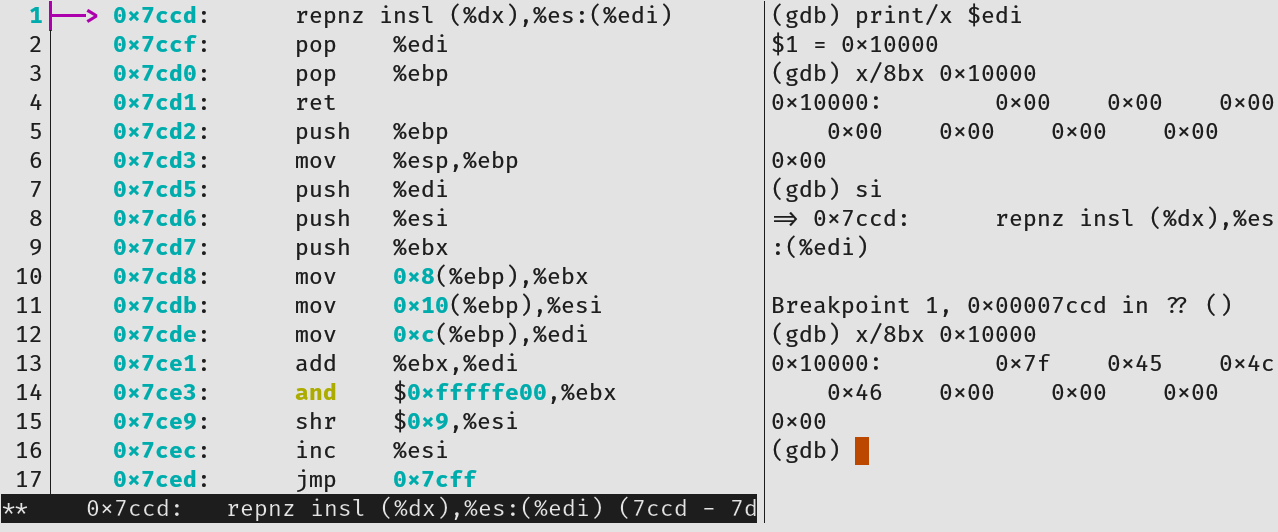
\includegraphics[width=0.9\linewidth]{lab1/exercise3_5.png}
    \caption{执行一条指令前后0x10000处的数据}
    \label{fig:exercise3_5}
\end{figure}
\par 可以看到,一条insl指令读取4字节的数据。因此读取一个扇区(512)字节的读取需要重复128次insl指令,执行到下一条指令时\%edi的值也验证了这一点。
\par 当读取完成后,执行如下三条指令,其作用是还原之前保护的寄存器的值并返回到调用者处。
\begin{lstlisting}
7ccf:	5f                   	pop    %edi
7cd0:	5d                   	pop    %ebp
7cd1:	c3                   	ret
\end{lstlisting}

\FloatBarrier
\par 回到readseg函数后,执行调用readsect完成后接下来的指令:
\begin{lstlisting}
    pa += SECTSIZE;
7cf6:	81 c3 00 02 00 00    	add    $0x200,%ebx
    offset++;
7cfc:	46                   	inc    %esi
7cfd:	58                   	pop    %eax
7cfe:	5a                   	pop    %edx
offset = (offset / SECTSIZE) + 1;

// If this is too slow, we could read lots of sectors at a time.
// We'd write more to memory than asked, but it doesn't matter --
// we load in increasing order.
while (pa < end_pa) {
7cff:	39 fb                	cmp    %edi,%ebx
7d01:	72 ec                	jb     7cef <readseg+0x1d>
\end{lstlisting}
\par 这些代码的作用在分析部分已经提到,其中0x7cf6和0x7cfc处的代码就是pa+=SECTSIZE以及offset++两条C语言代码的直接对应,紧随其后的两条pop则是释放先前传入readsect的参数。最后的cmp以及jb则实现了while循环。
\par 在while循环结束后的第一条语句打上断点,此处(0x7d03\textasciitilde 0x7d0a) 处的5条语句就是例行的恢复保护的寄存器以及返回到调用者处。之后,追踪返回到bootmain中。通过boot.asm可以判断出,在判断完ELF头部是否合法后,接下来的for语句的起始和结束位置分别为0x7d49以及0x7d5f\textasciitilde 0x7d61处。C语言for循环对应的汇编实现也是实现为do-while形式,与while类似,首先进行一次跳转。跳转到循环尾部再进行判断,如果判断成立则跳转到循环体开头处执行循环体,如果不是则直接执行下一语句,跳出循环。
\begin{lstlisting}
for (; ph < eph; ph++)
7d49:	eb 14                	jmp    7d5f <bootmain+0x54>
    // p_pa is the load address of this segment (as well
    // as the physical address)
    readseg(ph->p_pa, ph->p_memsz, ph->p_offset);
7d4b:	ff 73 04             	pushl  0x4(%ebx)
7d4e:	ff 73 14             	pushl  0x14(%ebx)
7d51:	ff 73 0c             	pushl  0xc(%ebx)
7d54:	e8 79 ff ff ff       	call   7cd2 <readseg>
    goto bad;

// load each program segment (ignores ph flags)
ph = (struct Proghdr *) ((uint8_t *) ELFHDR + ELFHDR->e_phoff);
eph = ph + ELFHDR->e_phnum;
for (; ph < eph; ph++)
7d59:	83 c3 20             	add    $0x20,%ebx
7d5c:	83 c4 0c             	add    $0xc,%esp
7d5f:	39 f3                	cmp    %esi,%ebx
7d61:	72 e8                	jb     7d4b <bootmain+0x40>
\end{lstlisting}
\par 0x7d4b\textasciitilde 0x7d59执行的就是for循环的循环体,也仅对应一条C语言语句,即readseg(ph->p\_pa, ph->p\_memsz, ph->p\_offset); 前面已经分析过readseg函数的执行过程,而这一语句,就是elfheader中所指向的信息加载到ph->p\_pa处。
\par 在循环执行完成后,只执行了一条语句:
\begin{lstlisting}
((void (*)(void)) (ELFHDR->e_entry))();
7d63:	ff 15 18 00 01 00    	call   *0x10018
\end{lstlisting}
\par 从C语言的语法分析,就是将ELFHDR->e\_entry强制转化为void (*)(void)类型的函数指针然后执行这一函数指针,也就是说,将CPU的控制权从bootloader转移给内核。在0x7d63处打上断点,进入内核后执行的第一条语句如\ref{fig:exercise3_6}所示。也就是0x10000c处的movw \$1234, 0x472。
\begin{figure}[htb]
    \centering
    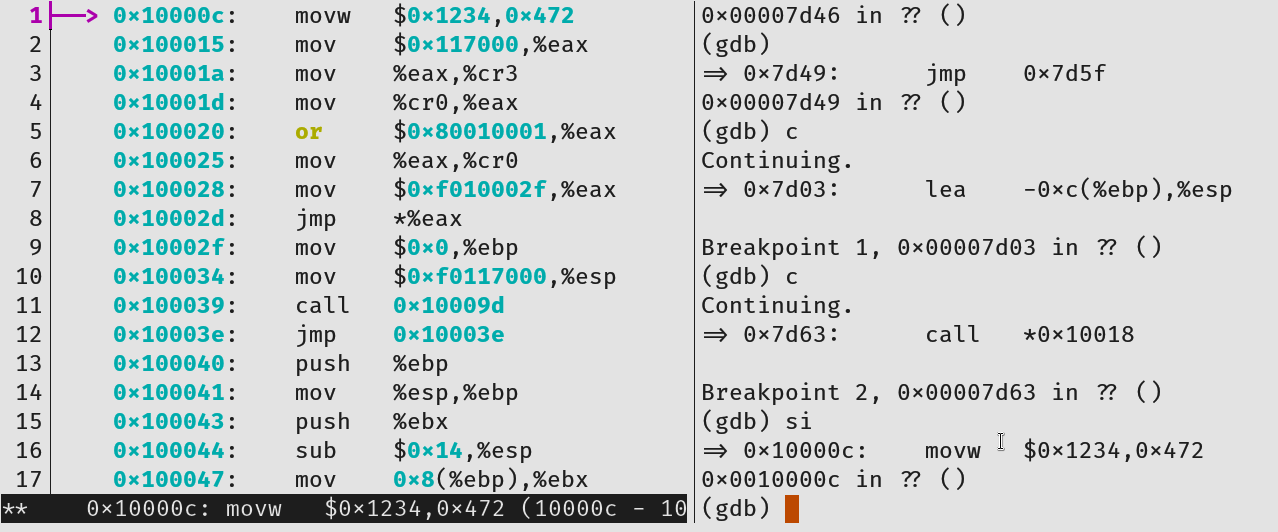
\includegraphics[width=0.9\linewidth]{lab1/exercise3_6.png}
    \caption{进入内核后执行的第一条语句}
    \label{fig:exercise3_6}
\end{figure}
\end{exerciseSolution}

\par 至此,对于整个bootloader的分析与追踪已经完成。对于实验指导中提出的4个问题,其答案在Exercise 3的分析与追踪的过程中已经给出:
\begin{enumerate}
    \item 在什么时候处理器开始工作于 32 位模式?是什么让 CPU 从 16 位模式切换到 32 位模式?
        \begin{itemize}
            \item 执行完0x7c2d处的ljmp \$0xb866, \$0x87c32(对应boot.S中ljmp \$PROT\_MODE\_CSEG, \$protcseg)语句后,处理器开始工作于32位模式。表面上,ljmp语句将CPU切换为32位模式,实际上是因为此时CPU工作于保护模式下。
        \end{itemize}
    \item boot loader 中执行的最后一条语句是什么?内核加载完成后执行的第一条语句又是什么?
        \begin{itemize}
            \item boot loader执行的最后一条语句是0x7d63处的call *0x10018,对应main.c中的 ((void (*)(void)) (ELFHDR->e\_entry))(); 这条语句执行完后,执行的第一条指令,也就是加载完内核后执行的第一条指令是movw \$0x1234, 0x472。
        \end{itemize}
    \item 内核的第一条指令在哪里?
        \begin{itemize}
            \item 内核的第一条指令在0x1000c处,对应的源码位于kern/entry.S 中。
        \end{itemize}
    \item boot loader 是如何知道他要加载多少扇区才能吧整个内核加载进入内存的?它是从哪里找到这些
        信息的?
        \begin{itemize}
            \item 这些信息位于操作系统的Program Header Table中,这个表存放在ELF Header中,通过读取这些信息就知道要读取多少扇区才能把整个内核送入内存。
        \end{itemize}
\end{enumerate}

\subsection{Loading the Kernel}
\par 在即进一步讨论boot loader的C语言部分之前先回顾一些有关C语言的基础知识。

\exercise{4}{
    \par 阅读并学习关于C语言指针的知识(最好的参考书籍是K\&R)。
    \par 阅读K\&R 5.1章到5.5章的内容,下载pointer.c\footnote{\url{https://pdos.csail.mit.edu/6.828/2017/labs/lab1/pointers.c}},然后编译运行它。确保你理解了所有打印出来的值是从哪里来的,尤其是第1行和第6行的指针以及第二行到第4行的值,以及为什么第5行的值看题来像是程序崩溃了。
}

\begin{exerciseSolution}{4}
\par 首先,下载,编译并运行poninters.c(编译为32位可执行文件),其过程如\ref{fig:exercise4_1}所示。
\begin{figure}[htb]
    \centering
    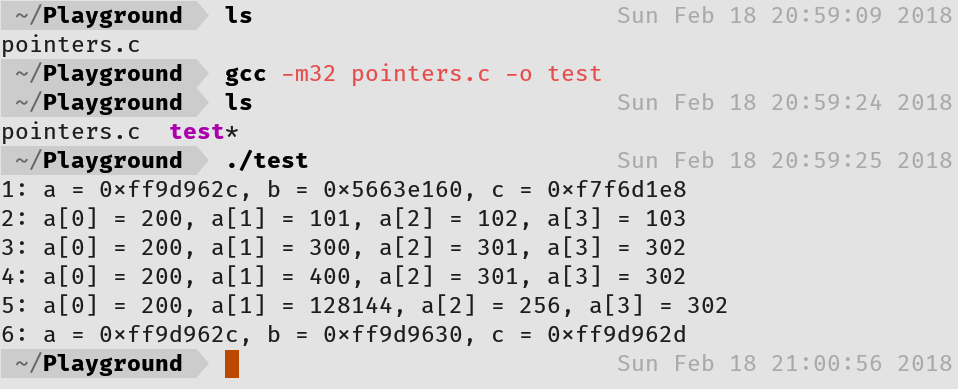
\includegraphics[width=0.8\linewidth]{lab1/exercise4_1.png}
    \caption{编译pointers.c以及运行的过程}
    \label{fig:exercise4_1}
\end{figure}

\par 观察源程序。首先程序声明了1个数组int a[4]、2个指针int *b, int *c以及一个整形值i。然后执行了第一条语句:
\inputCodeSetLanguage{c}
\begin{lstlisting}
printf("1: a = %p, b = %p, c = %p\n", a, b, c);
\end{lstlisting}
\par 显然,输出的a,b,c分别为a的首地址0xff9d962c,molloc为b分配的地址0x5663e160以及未初始化的指针c的地址0xf7f6d1e8。

\par 在此之后直到打印第二行之前,执行了如下的语句:
\begin{lstlisting}
c = a;
for (i = 0; i < 4; i++)
    a[i] = 100 + i;
c[0] = 200;
\end{lstlisting}
\par 首先,让指针c指向a的首地址,然后使用一个for语句令数组a的四个元素的值变为100, 101, 102, 103, 最后,将c[0]置为200。由于c只想的即a的首地址,因此修改的就是a[0]的值,因此a[0] = 200。a[1], a[2], a[3]的值维持不变。

\par 然后直到打印第三行之前,执行了如下语句:
\begin{lstlisting}
c[1] = 300;
*(c + 2) = 301;
3[c] = 302;
\end{lstlisting}
\par 这是c语言访问数组的3中不同的方法。由于在前一步中已经将c指向数组a的首地址,因此此处修改c[1], *(c+2), 3[c]的值实际上就是在修改a[1], a[2], a[3]的值。修改完成后a[1]=300, a[2]=301, a[3]=302。

\par 在打印第4行之前执行的语句为:
\begin{lstlisting}
c = c + 1;
*c = 400;
\end{lstlisting}
\par 这两条语句将c指向了a[1]所在的地址并修改了c所在地址处的值。即将a[1]修改为了400,a[0], a[2], a[3]的值没有变。

\par 在打印第5行之前执行的语句为:
\begin{lstlisting}
c = (int *) ((char *) c + 1);
*c = 500;
\end{lstlisting}
\par 第一句:首先将int型指针c强制转换为char型指针,然后将此指针值加上1,然后再强制转换回int型指针。从图\ref{fig:exercise4_1}可以推断出,在执行这一语句前a[1]的地址为0xff9d962c+0x4=0xff9d9630,强制转换为char型指针后加上1,得到的值为0xff9d9631(加上了一个char的大小),然后再强制转换回int型指针。又由于x86CPU采用的是小端存储,因此此时修改*c的值相当于修改了a[1]的高3个字节以及a[2]的最低字节,分别修改为500的低3个字节以及500的最高字节。因此修改后a[1]=128144, a[2]=256, a[0]和a[3]不变,修改前后各个字节的值如表\ref{tab:4_1}所示。
\begin{table}[htp]
    \centering
    \caption{a[1]以及a[2]各字节变换}
    \label{tab:4_1}
    \begin{tabular}{r c c c c c c c c}
        \toprule
        数组 & \multicolumn{4}{c}{a[1]} & \multicolumn{4}{c}{a[2]}\\
        \cmidrule(lr){2-5} \cmidrule(lr){6-9}
        地址(偏移量0xff9d9600) & 0x30 & 0x31 & 0x32 & 0x33 & 0x34 & 0x35 & 0x36 & 0x37 \\
        值(更改前)& 90   & 01   & 00   & 00   & 2d   & 01   & 00   & 00   \\
        值(更改后)& 90   & \textbf{f4} & \textbf{01 } & \textbf{00} & \textbf{00} & 01 & 00 & 00  \\
        \bottomrule
    \end{tabular}
\end{table}

\par 在打印最后一行前执行的操作为:
\begin{lstlisting}
b = (int *) a + 1;
c = (int *) ((char *) a + 1);
\end{lstlisting}
\par 这两条语句将指针b指向a[1]的地址,将指针c再按照打印第5行的方法加设置为a[0]的地址上1个char的长度。于是指针b的值变为0xff9d9630,指针c的值变为0xff9d962d。
\end{exerciseSolution}

\par 为了能够理解boot/main.c,首先需要知道ELF文件的结构。ELF文件由3部分组成:带有加载信息的文件头,程序段表以及程序段。每一个段都是一块连续的代码或者数据。它们在运行时首先要被加载到内存中,而boot loader的任务就是要把它们加载到内存中。对于jOS而言,我们对3个段非常感兴趣:
\begin{itemize}
    \item .text段:存放程序的可执行代码
    \item .rodata段,存放所有的只读数据,如字符串常量
    \item .data段,存放所有被初始化后的数据段,比如有初值的全局变量。
\end{itemize}

\par 通过objdump命令可以得到有关这些段的信息。运行objdump -h obj/kern/kernel命令后得到如下结果:

\inputCodeSetLanguage{bash}
\begin{lstlisting}[numbers=none]
   obj/kern/kernel:     file format elf32-i386

Sections:
Idx Name          Size      VMA       LMA       File off  Algn
  0 .text         0000178e  f0100000  00100000  00001000  2**2
                  CONTENTS, ALLOC, LOAD, READONLY, CODE
  1 .rodata       00000704  f01017a0  001017a0  000027a0  2**5
                  CONTENTS, ALLOC, LOAD, READONLY, DATA
  2 .stab         000044e9  f0101ea4  00101ea4  00002ea4  2**2
                  CONTENTS, ALLOC, LOAD, READONLY, DATA
  3 .stabstr      00008c34  f010638d  0010638d  0000738d  2**0
                  CONTENTS, ALLOC, LOAD, READONLY, DATA
  4 .data         0000a300  f010f000  0010f000  00010000  2**12
                  CONTENTS, ALLOC, LOAD, DATA
  5 .bss          00000644  f0119300  00119300  0001a300  2**5
                  ALLOC
  6 .comment      00000011  00000000  00000000  0001a300  2**0
                  CONTENTS, READONLY
\end{lstlisting}
\par 可以看出,其中不仅仅包含.text, .rodata以及.data段,还包含一些其他的段信息。在这些信息中对于每一个段都有一个VMA以及一个LMA,VMA就是这个段的逻辑地址,而LMA则为这个段被加载到内存后的物理地址。

\par 通过objdump -x obj/kern/kernl命令,我们可以看到ELF中哪些部分将被加载到内存,以及被加载到内存中的哪个地址,其输出如下:
\begin{lstlisting}[numbers=none]
obj/kern/kernel:     file format elf32-i386
obj/kern/kernel
architecture: i386, flags 0x00000112:
EXEC_P, HAS_SYMS, D_PAGED
start address 0x0010000c

Program Header:
    LOAD off    0x00001000 vaddr 0xf0100000 paddr 0x00100000 align 2**12
    filesz 0x0000efc1 memsz 0x0000efc1 flags r-x
    LOAD off    0x00010000 vaddr 0xf010f000 paddr 0x0010f000 align 2**12
    filesz 0x0000a300 memsz 0x0000a944 flags rw-
...
\end{lstlisting}
\par Program Header中列出的就是所有被加载到内存中的段的信息,也就是Program Headers Table 中的表项,所有而需要被加载到内存的段都被标记为LOAD。BIOS会把boot sector加载到0x7c00处,这是boot sector的加载地址,也是其链接地址。我们可以通过boot/Makefrag中的-Ttext修改链接地址。

\exercise{5}{
    \par 再次追中进入boot loader然后尝试辨认出哪些语句会在boot loader的链接地址变化后``坏掉''。在boot/Makefrag中修改链接地址为一个错误的地址,然后运行make clean。用make重新编译整个lab,并追踪进boot loader看发生了什么。最后别忘了把链接地址改回来并运行make clean。
}

\begin{exerciseSolution}{5}
\par 首先,运行make clean将之前的编译结果清除掉,然后修改boot/Makefrag中的链接地址。Makefrag中,文件\$(OBJDIR)/boot/boot的编译命令中-Ttext 0x7C00即为链接地址。将其修改为0x1000后重新运行make 进行编译。编译完成后obj/boot/boot.asm中程序的前数行如下:
\inputCodeSetLanguage{[x86masm]Assembler}
\begin{lstlisting}
.globl start
start:
  .code16                     # Assemble for 16-bit mode
  cli                         # Disable interrupts
    1000:	fa                   	cli
  cld                         # String operations increment
    1001:	fc                   	cld
\end{lstlisting}
\par 可以看出,程序的虚拟地址已经从的0x1000而不是0x7c00开始了。BIOS仍然会把boot loader加载到0x7c00处,因此在0x7c00处打上打断点并调试。执行到断点后,gdb显示如图\ref{fig:exercise5_1}所示。可以看到,前几句程序依然是正常执行。
\begin{figure}[htb]
    \centering
    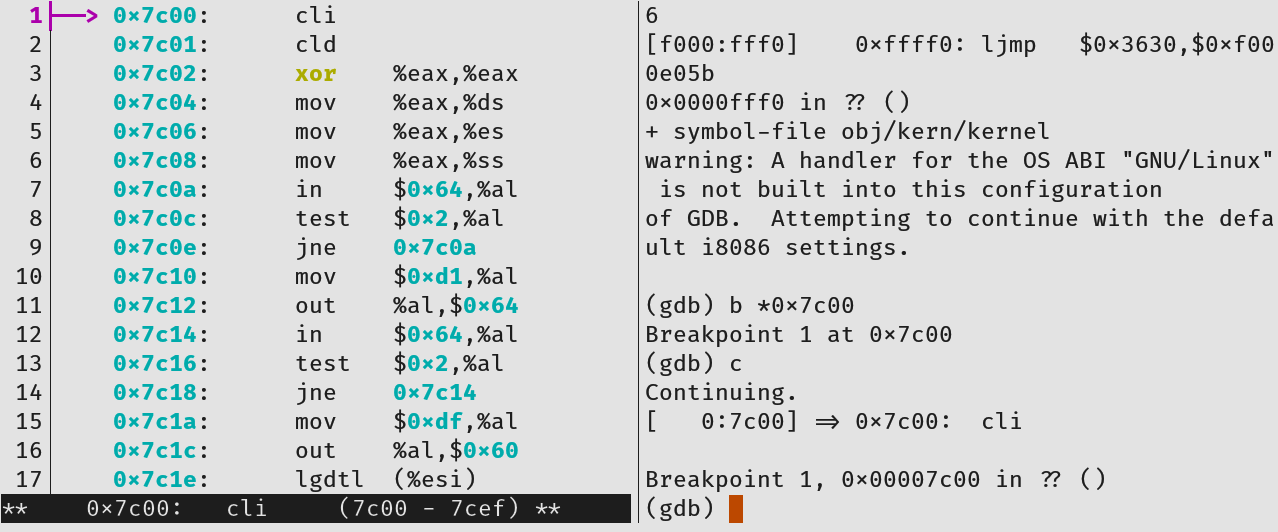
\includegraphics[width=0.9\linewidth]{lab1/exercise5_1.png}
    \caption{重新编译后执行到断点时的gdb显示}
    \label{fig:exercise5_1}
\end{figure}
\par 接下来单步执行,在执行到ljmp指令时,本应该直接执行ljmp的下一条指令地址,但是这里由于链接地址的错误直接跳转到了0xe05b,如\ref{fig:exercise5_2}所示,导致了错误,程序不能够继续运行。
\begin{figure}[htb]
    \centering
    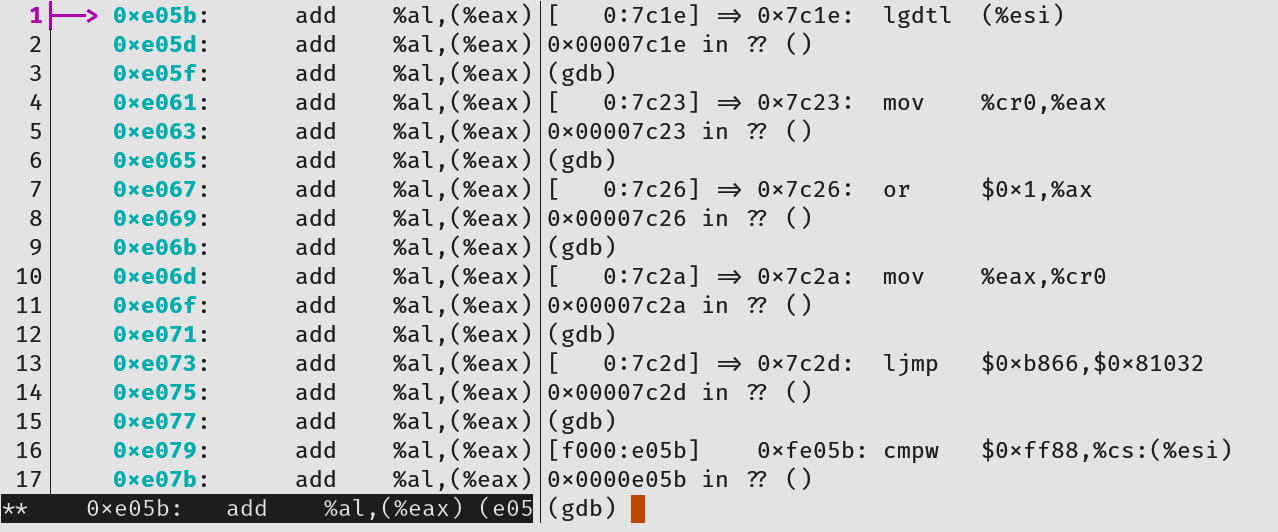
\includegraphics[width=0.9\linewidth]{lab1/exercise5_2.png}
    \caption{ljmp指令跳转后gdb显示}
    \label{fig:exercise5_2}
\end{figure}
\end{exerciseSolution}

\par 对于内核而言,其加载地址和链接地址是不同的。这和boot loader不一样。bootloader将内核加载在低地址处,但是内核运行在高地址处。通过objdump -f obj/kern/kernel可以看到ELF头部中的e\_entry字段。这个字段存放的就是可执行程序入口的链接地址。这一命令输出如下:
\inputCodeSetLanguage{bash}
\begin{lstlisting}[numbers=none]
obj/kern/kernel:     file format elf32-i386
architecture: i386, flags 0x00000112:
EXEC_P, HAS_SYMS, D_PAGED
start address 0x0010000c
\end{lstlisting}

\exercise{6}{
    \par 使用GDB的x命令可以检查内存中的内容。使用x/Nx ADDR可以查看ADDR处的N个字的内容。字的大小是没有一个标准的,但是在GDB中,一个字为2个字节。重置机器(退出QEMU/GDB并重启,然后分别在BIOS进入bootloader以及bootloader进入kernel时检查0x00100000处的8个字。为什么这些内容是不同的?第二个断点处的内容是什么?
}

\begin{exerciseSolution}{6}
\par 首先重新编译并启动qemu/gdb,然后在0x7c00处打上断点。运行到断点处,使用x/8x 0x00100000命令检查0x00100000处的8个字。其结果如图\ref{fig:exercise6_1}所示。
\begin{figure}[htb]
    \centering
    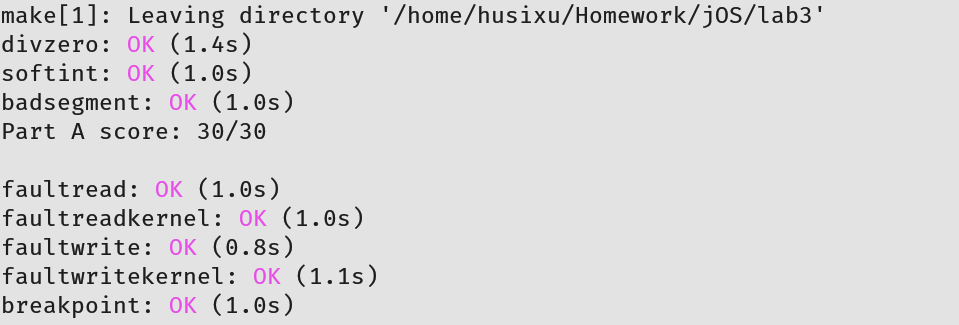
\includegraphics[width=0.9\linewidth]{lab1/exercise6_1.png}
    \caption{从BIOS进入boot loader后0x00100000处的内容}
    \label{fig:exercise6_1}
\end{figure}

\par Exercise 3告诉我们,从boot loader进入内核后执行的第一条指令在0x10000c处,因此在0x10000c处打上断点。运行到这一断点并重新使用x/8x 0x00100000检查,其结果如图\ref{fig:exercise6_2}所示。
\begin{figure}[htb]
    \centering
    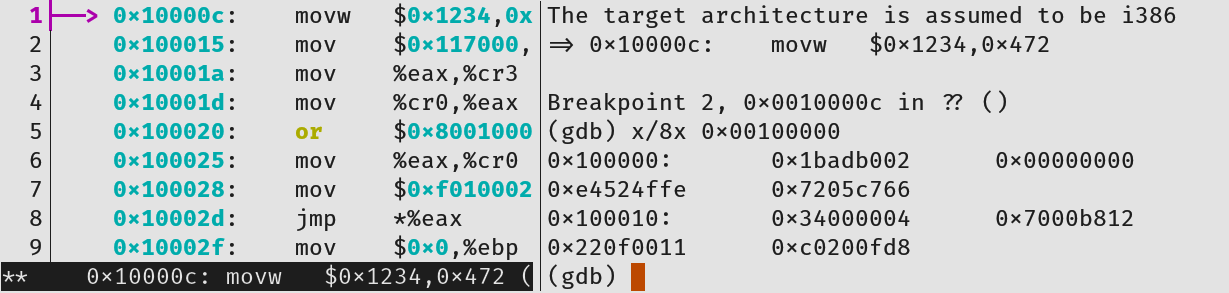
\includegraphics[width=0.9\linewidth]{lab1/exercise6_2.png}
    \caption{从boot loader进入内核后0x00100000处的内容}
    \label{fig:exercise6_2}
\end{figure}

\FloatBarrier
\par 观察obj/kern/kernel.asm的前几条指令,其指令内容如下:
\inputCodeSetLanguage{[x86masm]Assembler}
\begin{lstlisting}
.globl entry
entry:
        movw	$0x1234,0x472			# warm boot
f0100000:	02 b0 ad 1b 00 00    	add    0x1bad(%eax),%dh
f0100006:	00 00                	add    %al,(%eax)
f0100008:	fe 4f 52             	decb   0x52(%edi)
f010000b:	e4 66                	in     $0x66,%al

f010000c <entry>:
f010000c:	66 c7 05 72 04 00 00 	movw   $0x1234,0x472
f0100013:	34 12
\end{lstlisting}
\par 可以看出,gdb中0x00100000处的内容与此处的内容一致。此时可以回答Exercise 6提出的两个问题:此处内容不同是因为boot loader将内核加载到了0x00100000处,这8个字的内容就是内核的前若干条指令。
\end{exerciseSolution}

\FloatBarrier
\section{The Kernel}
\subsection{Using virtual memory to work around position dependence}
\par 在使用boot loader时,链接地址和加载地址是一样的,也就是说虚拟地址和物理地址是一样的。但是进入到内核程序后这两种地址就不再相同了。内核的虚拟地址会被链接到一个非常高的地址空间,对于jOS而言是0xf0100000。剩下的较低部分的空间给其他的用户程序使用。
\par 但是由于许多机器没有0xf0100000的物理内存,因此在运行的时候需要把虚拟地址映射到物理地址0x00100000处运行。此时加载的物理地址仅仅高于BIOS ROM。此时PC仅最少需要1MB物理内存。
\par 在这个实验中,采用分页管理的方法来实现映射,但是不是使用的通常的分页管理器,而是自己写了一个lab/kern/entrygdir.c进行映射。因此其功能很简单,只能够把0x00000000\textasciitilde 0xf0400000以及0x00000000\textasciitilde 0x00400000映射到0x0000000\textasciitilde 0x0-0400000的范围内。不再这两个虚拟地址范围内的地址都会引起硬件异常。

\exercise{7}{
    \par 使用QEMU和GDB跟踪进入JOS的内核,并停在movl \%eax, \%cr0处,检查0x00100000处的内容以及0xf0100000处的内容。现在用stepi单步执行这个命令然后再检查0x00100000处的内容和0xf0100000处的内容,并确保你弄懂了刚才发生了什么。
    \par 如果不能正常建立映射,在新映射建立后最先不能够正常工作的指令是哪一条?注释掉kern/entry.S中的movl \%eax, \%cr0指令,然后看看你是否是正确的。
}

\begin{exerciseSolution}{7}
\par 启动qemu和gdb,由于Exercise 3已知程序的入口是0x10000c,因此首先在0x10000c处打上断点并运行到0x10000c处,然后使用x/8x检查0x00100000和0xf100000处的内容,其内容如图\ref{fig:exercise7_1}所示。
\begin{figure}[htb]
    \centering
    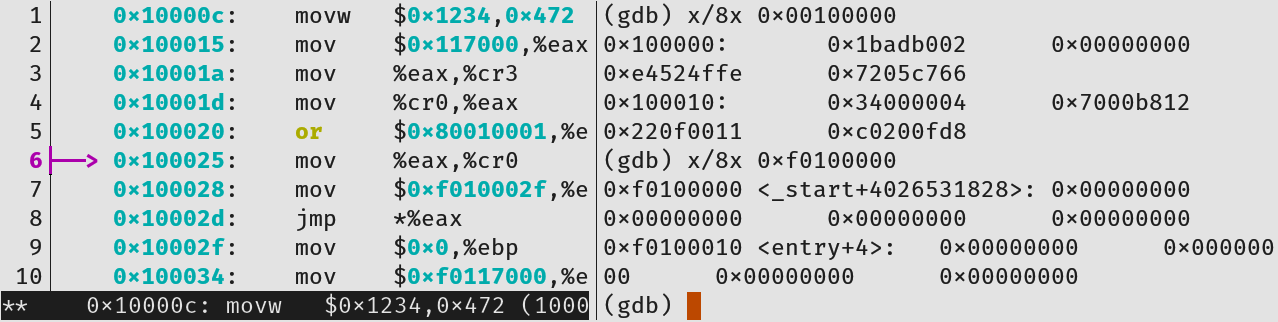
\includegraphics[width=0.9\linewidth]{lab1/exercise7_1.png}
    \caption{执行movl \%eax, \%cr0前的两处内存中的内容}
    \label{fig:exercise7_1}
\end{figure}
\par 由Exercise 6已知,0x00100000处的内容就是内核的前几条指令,而从图\ref{fig:exercise7_1}中可知,0xf0100000 处的内容全为0。继续执行一步stepi以后,在次运行两个x/8x指令,这时显示的内容如\ref{fig:exercise7_2}所示。
\begin{figure}[htb]
    \centering
    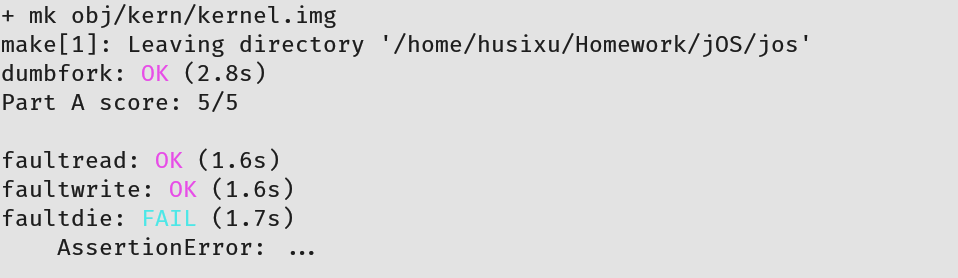
\includegraphics[width=0.9\linewidth]{lab1/exercise7_2.png}
    \caption{执行movl \%eax, \%cr0后的两处内存中的内容}
    \label{fig:exercise7_2}
\end{figure}
\par 可以看出,在执行了movl \%eax, \%cr0指令以后,两处的内容完全相同。这说明了此时已经成功启用了页表并完成了地址映射。
\par 下面注释掉movl \%eax, \%cr0,make clean之后重新编译运行。逐步使用stepi之后在一个jmp指令后出现了问题,如图\ref{fig:exercise7_3}。0x10002a处的jmp指令需要跳转到0xf010002c处,但是没有分页管理不会进行虚拟地址映射到物理地址的转化,因此访问超出内存限制后程序崩溃。
\begin{figure}[htb]
    \centering
    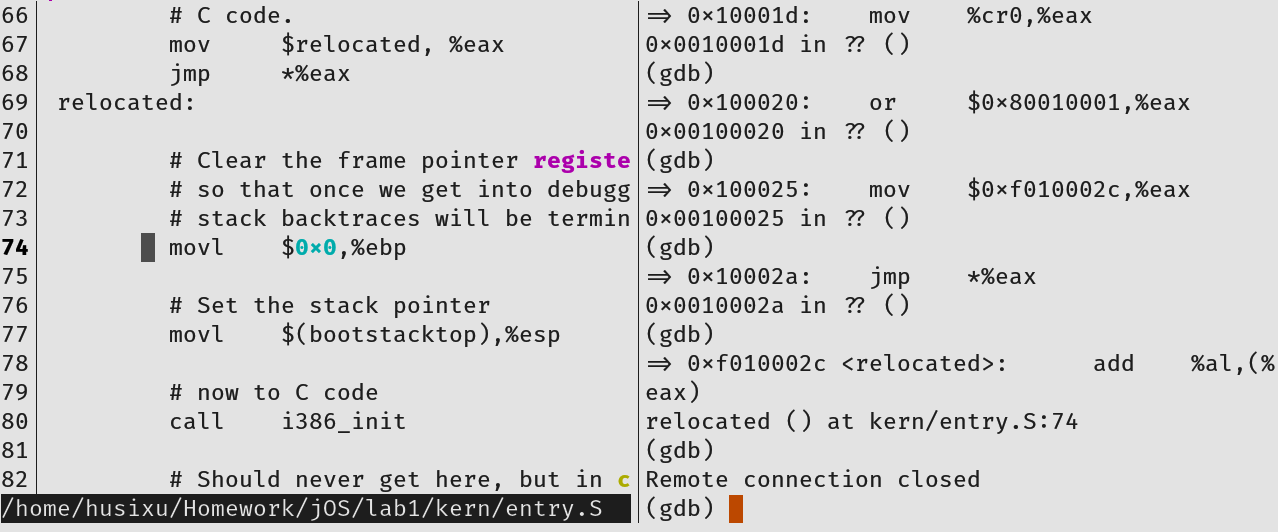
\includegraphics[width=0.9\linewidth]{lab1/exercise7_3.png}
    \caption{jmp指令后程序崩溃}
    \label{fig:exercise7_3}
\end{figure}
\FloatBarrier
\end{exerciseSolution}

\subsection{Formatted Printing to the Console}
\par 阅读kern/printf.c,lib/printfmt.c和kern/console.c的代码,分析他们之间的关系。

\exercise{8}{
    \par 有一小部分用于打印八进制数(``\%o''格式)的代码被遗漏了,找出并补全这部分程序。
}
\begin{exerciseSolution}{8}
\par 要进行这个练习首先要分析kern/printf.c,kern/console.c以及lib/printfmt.c之间的关系。初步观察3个文件,发现kern/printf.c中的cprintf, vprintf函数调用了lib/printfmt.c中的vprintfmt函数。kern/printf.c中的putch程序和lib/printfmt程序调用了kern/console.c中的cputchar程序。进一步使用静态分析工具进行分析,cprintf的调用关系图(call graph)如图\ref{fig:exercise8_1}所示。
\begin{figure}[htb]
    \centering
    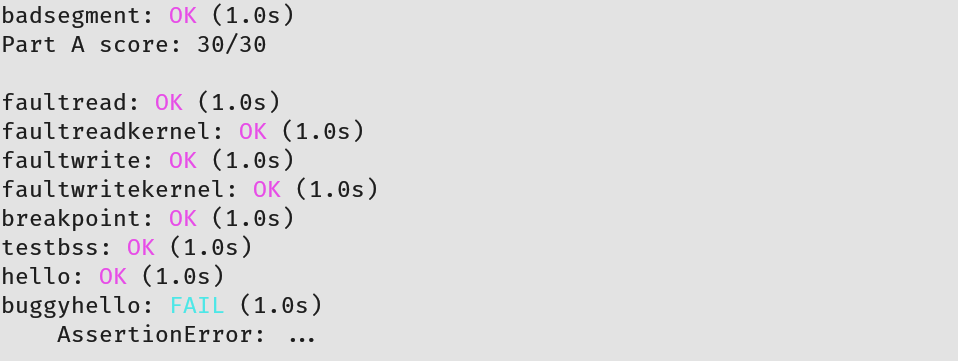
\includegraphics[width=0.9\linewidth]{lab1/exercise8_1.png}
    \caption{cprintf的调用关系图}
    \label{fig:exercise8_1}
\end{figure}

\par 首先可以看到,这些函数中最接近底层的是cons\_putc,通过它的注释可以看到cons\_putc的作用是输出一个字符到控制台。而cons\_putc是通过调用serial\_putc,lpt\_putc以及cga\_putc实现的。serial\_putc的代码及有关常量定义如下:
\inputCodeSetLanguage{c}
\begin{lstlisting}
#define COM1          0x3F8
#define COM_LSR       5    // In:    Line Status Register
#define COM_LSR_TXRDY 0x20 //   Transmit buffer avail
#define COM_TX        0    // Out: Transmit buffer (DLAB=0)

static void serial_putc(int c) {
    int i;
    for (i = 0; !(inb(COM1 + COM_LSR) & COM_LSR_TXRDY) && i < 12800; i++)
        delay();
    outb(COM1 + COM_TX, c);
}
\end{lstlisting}
\par 通过查询端口功能\footnote{\url{http://bochs.sourceforge.net/techspec/PORTS.LST}},并分析代码,发现代码\lstinline{!(inb(COM1 + COM_LSR) & COM_LSR_TXRDY)}是用于检测03FD的bit5是否为1,而这一位用于判断发送数据缓冲区寄存器是否为空。outb则是向03F8发送数据c而03F8被写入时功能为发送数据到串口。因此serial\_putc的作用是向串口发送一个字符。
\par 通过同样的方法,可以判断处lpt\_putc的作用是向并口发送这个字符。最后,cga\_putc的作用是向cga设备,也就是计算机的显示器发送一个字符。cga\_putc对于需要输出的字符进行判断,如果是如'\textbackslash t'、'\textbackslash b'等特殊字符则移动光标的位置或者执行相应动作,否则直接将字符显示输出在屏幕上。switch后面的if用于判断缓冲区显示的内容不能够超过显示器大小CRT\_SIZE。
\par 向上分析,cputchar直接调用cons\_putc,而putchar直接调用cputchar,并将计数器加一计数。vprintfmt则调用cputc进行打印输出。printfmt则是帮助vprintfmt进行递归调用的一个帮助函数。观察vprintfmt,发现其由4个参数:
\begin{enumerate}
    \item void (*putch)(int, void*)是一个输出一个字符的函数指针。其第二个地址是字符输出位置的地址的地址,由于需要实现将值输出到这个地址后地址+1,因此这个函数指针的第二个参数不是地址而是地址的地址。
    \item void *putdat是这个字符要存放的内存地址指针
    \item const char* fmt是输入的格式化字符串
    \item va\_list ap是格式化字符串的可变长参数。
\end{enumerate}
\par 这个vprintfmt函数就是需要被修改的函数,将输出八进制的部分修改为如下代码即可实现8进制输出。
\begin{lstlisting}
    case 'o':
        num = getuint(&ap, lflag);
        base = 8;
        goto number;
\end{lstlisting}
\par 修改完成以后重新编译,即在命令行中执行make clean \&\& make \&\& make qemu以后,qemu启动后会出现一行说明修改成功的输出:6828 decimal is 15254 octal!,如图\ref{fig:exercise8_2}所示。
\begin{figure}[htb]
    \centering
    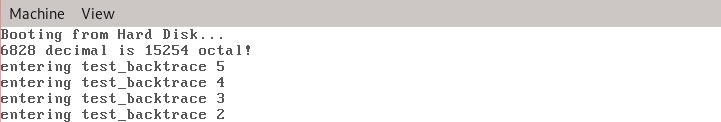
\includegraphics[width=0.9\linewidth]{lab1/exercise8_2.png}
    \caption{重新编译并启动qemu后的部分输出}
    \label{fig:exercise8_2}
\end{figure}

\FloatBarrier
\end{exerciseSolution}

\par 接下来对于实验指导中Exercise 8之后的问题,给出解答。
\begin{enumerate}
    \item 解释printf.c和console.c之间的接口,尤其是console.c导出了那个函数?这个函数是如何在printf.c中被使用的?
        \begin{itemize}
            \item 在Exercise 8中已经给出分析部分。console.c中除了静态函数之外所有的函数都导出并为外部提供服务了。printf.c调用console.c中的cputchar函数进行显示输出。
        \end{itemize}
    \item 解释如下console.c中的代码:
        \inputCodeSetLanguage{c}
        \begin{lstlisting}[gobble=12]
            if (crt_pos >= CRT_SIZE) {
                int i;
                memmove(crt_buf, crt_buf + CRT_COLS, (CRT_SIZE - CRT_COLS) * sizeof(uint16_t));
                for (i = CRT_SIZE - CRT_COLS; i < CRT_SIZE; i++)
                    crt_buf[i] = 0x0700 | ' ';
                crt_pos -= CRT_COLS;
            }
        \end{lstlisting}
        \begin{itemize}
            \item 这部分代码是为了当输出超过显示屏的大小的时候将显示屏向上滚动一行,由于显示屏大小为$80\times 25$,因此将1\textasciitilde 24行复制并放在0\textasciitilde 23行,然后将最后一行清空。mmove的作用是滚动,而for循环的作用是清空最后一行。
        \end{itemize}
    \item 单步执行如下代码:
        \begin{lstlisting}[gobble=12]
            int x = 1, y = 3, z = 4;
            cprintf("x %d, y %x, z %d\n", x, y, z);
        \end{lstlisting}
        \begin{enumerate}
            \item 在调用cprintf的过程中,fmt指向那里?ap指向哪里?
            \item 按照执行的顺序列出对于cons\_putc, va\_arg, 以及vcprintf的调用。对于cons\_putc,列出它的参数。对于va\_arg,列出调用前后ap指向哪里。对于vcprintf列出它的两个参数的值。
        \end{enumerate}
        \begin{itemize}
            \item 在kern/monitor.c中的mon\_backtrace中添加这两条语句并打开gcc进行追踪,发现fmt指向格式化字符串"x \%d, y\%x, z\%n",而ap指向参数x, y, z,如图\ref{fig:exercise8_3}所示。(由于在cprintf中不能正常看到fmt以及ap的值因此实际取值实在vcprintf中进行的。
                \begin{figure}[htb]
                    \centering
                    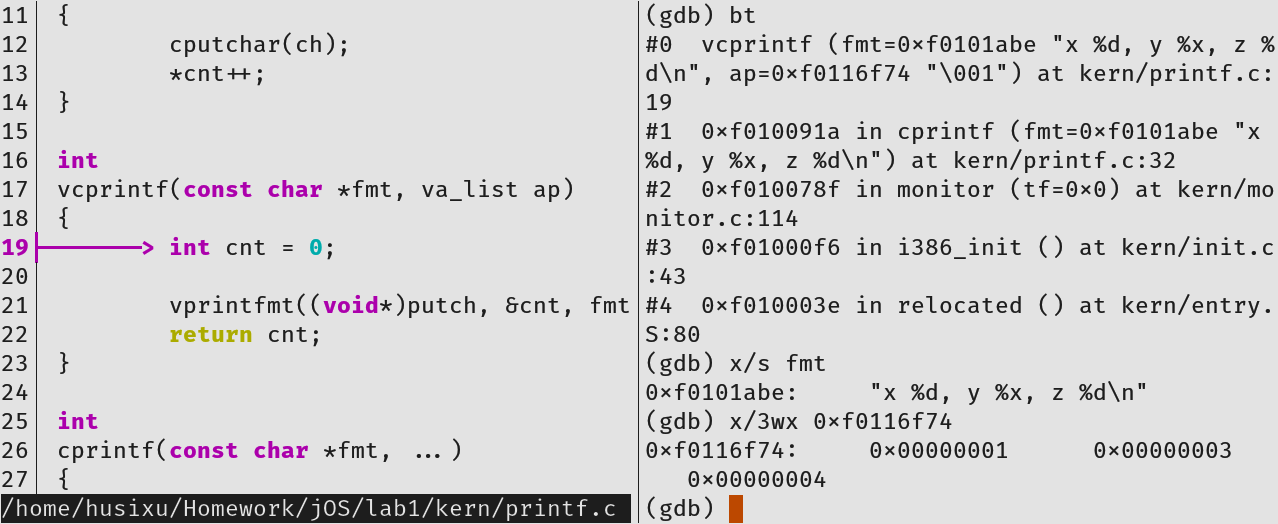
\includegraphics[width=0.9\linewidth]{lab1/exercise8_3.png}
                    \caption{fmt以及ap的取值}
                    \label{fig:exercise8_3}
                \end{figure}
            \item 通过对于代码的跟踪,可以得知按照顺序,对于三个函数的调用过程如表\ref{tab:8_1}所示。
            \item 对于这三个函数的调用,getint使用va\_arg根据不同的参数类型从参数列表中取出下一个参数。第一次对于va\_arg进行调用前ap为1,3,4,调用后变为3,4。最后,所有函数的调用顺序如表\ref{tab:8_1}所示。
                \begin{table}[H]
                    \centering
                    \caption{vcprintf, va\_arg以及cons\_putc的调用顺序}
                    \label{tab:8_1}
                    \begin{tabular}{c r l}
                        \toprule
                        \multicolumn{1}{c}{\textbf{\#}} &
                        \multicolumn{1}{c}{\textbf{函数}} &
                        \multicolumn{1}{c}{\textbf{备注}} \\
                        \cmidrule(lr){1-3}
                        1  & vcprintf  & fmt=``x \%d, y \%x, z \%d \textbackslash n'', ap=1,3,4 \\
                        2  & cons\_putc & c=120 \\
                        3  & cons\_putc & c=32  \\
                        4  & va\_arg    & 调用前 ap=1,3,4 调用后ap=3,4 \\
                        5  & cons\_putc & c=49  \\
                        6  & cons\_putc & c=44  \\
                        7  & cons\_putc & c=32  \\
                        8  & cons\_putc & c=121 \\
                        9  & cons\_putc & c=32  \\
                        10 & va\_arg    & 调用前 ap=3,4 调用后ap=4 \\
                        11 & cons\_putc & c=51  \\
                        12 & cons\_putc & c=44  \\
                        13 & cons\_putc & c=32  \\
                        14 & cons\_putc & c=122 \\
                        15 & cons\_putc & c=32  \\
                        16 & va\_arg    & 调用前 ap=4 调用后ap为空 \\
                        17 & cons\_putc & c=52  \\
                        18 & cons\_putc & c=10  \\
                        \bottomrule
                    \end{tabular}
                \end{table}
        \end{itemize}
    \item 运行如下代码:
        \begin{lstlisting}[gobble=12]
            unsigned int i = 0x00646c72;
            cprintf("H%x Wo%s", 57616, &i);
        \end{lstlisting}
        输出是什么?按照上一题的方法逐步解释输出是怎么来的。输出依赖于x86系统是小端这一事实。如果x86是大端的,当i为何值时才会有相同的输出?你需要将57616更改为一个不同的值吗?
        \begin{itemize}
            \item 与上一题类似,首先,将这两句代码加入monitor.c中,然后重新编译并运行,最后得到的运行结果为``He110, World'',如图\ref{fig:exercise8_4}所示。
                \begin{figure}[htb]
                    \centering
                    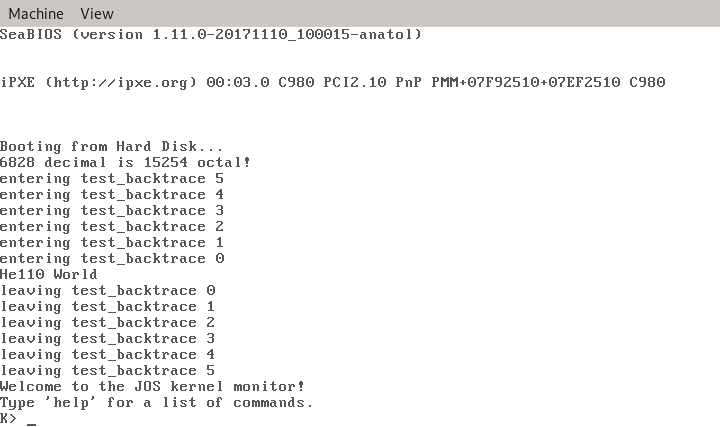
\includegraphics[width=0.6\linewidth]{lab1/exercise8_4.png}
                    \caption{重新编译后的运行结果}
                    \label{fig:exercise8_4}
                \end{figure}
                \par 输出这个值的原因是:第一个\%x要求按照16进制输出第一个参数,而第一个参数的值为57616,对应的16进制为e110,因此前半部分输出为He110,而第二个格式化字符\%s要求将\&i作为一个字符串输出,此时将i进行拆分。由于x86是小端模式,因此地址由低向高增长时字节也由LSB向MSB增长。因此将0x00646c72拆分后,变为0x72('r'), 0x6c('l'), 0x54('d'), 0x00('\textbackslash 0')。于是后半部分输出World。当i是大端时,需要能够将i改为0x726c6400才能有相同的输出,但是不需要改变57616这个值。
        \end{itemize}
    \item 在接下来的代码中,`y='之后打印的是什么?(注意:答案不是一个特定值。)这为什么会发生?
        \begin{lstlisting}[gobble=12]
            cprintf("x=%d y=%d", 3);
        \end{lstlisting}
        \begin{itemize}
            \item 同样的,将这个代码输入monitor.c后重新编译运行,输出的结果为``x=3 y=-267292872'',x后面输出的为3,因为第一个参数为3,而y没有指定参数,因此将输出一个不确定的值,实际上,是从栈中3这个参数的后方多取了一个数作为参数。
        \end{itemize}
    \item 让我们假设GCC改变了函数调用转换,并将参数入栈顺序更改为声明顺序,也就是说最后一个参数最后入栈。你需要如何更改cprintf或它的接口才能使传递任意参数仍然可行?
        \begin{itemize}
            \item 将变长参数置于格式化字符串的前方即可,即将cprintf的接口变为 \lstinline{int cprintf(..., const char *fmt)}。
        \end{itemize}
\end{enumerate}

\subsection{The Stack}
\par 这一份将重新编写一个kernel monitor程序用于记录堆栈的变化,该变化是由一系列被保存到堆栈的IP寄存器的值组成的。

\exercise{9}{
    \par 判断操作系统的内核从哪一条指令开始初始化它的堆栈空间,以及这个堆栈空间在内存的哪个地方?内核是如何给堆栈保留一块内存空间的?堆栈指针是指向这个区域的哪一端的?
}
\begin{exerciseSolution}{9}
    \par 在进入内核之前,整个boot loader是没有对\%esp和\%ebp的内容进行修改的,因此这其中没有初始化堆栈空间的语句。而在entry.S中,发现其最后几条指令如下:
    \inputCodeSetLanguage{[x86masm]Assembler}
    \begin{lstlisting}
relocated:
    # Clear the frame pointer register (EBP)
    # so that once we get into debugging C code,
    # stack backtraces will be terminated properly.
    movl	$0x0,%ebp			# nuke frame pointer

    # Set the stack pointer
    movl	$(bootstacktop),%esp

    # now to C code
    call	i386_init
    \end{lstlisting}
    \par 通过最后一条指令跳转到C函数中,以及前两条语句的注释可以判断,movl \$0x0,\%ebp以及movl \$(bootstacktop),\%esp就是用于初始化堆栈空间的语句。这两条语句中,第一条将0赋值给\%ebp,第二条将\$(bootstacktop)赋值给\%esp,此时需要进入gdb进行调试。当执行到这两条指令时,gdb显示如图\ref{fig:exercise9_1}所示。
    \begin{figure}[htb]
        \centering
        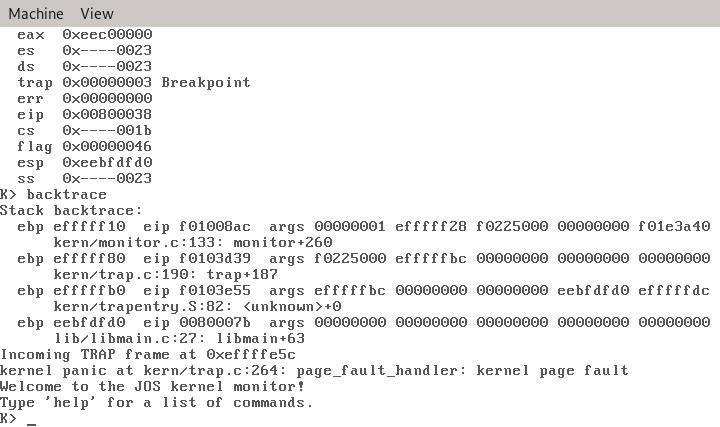
\includegraphics[width=0.9\linewidth]{lab1/exercise9_1.png}
        \caption{gdb显示输出}
        \label{fig:exercise9_1}
    \end{figure}
    \par 从图中可以发现,movl \$(bootstacktop),\%esp在运行时为mov \$0xf0117000,\%esp。也就是说栈顶的地址为0xf0117000。而根据entry.S最后的标志可以发现,在栈顶前分配了KSTKSIZE这么多的空间。 KSTKSIZE在inc/memlayout.h中定义。其大小为(8*PGSIZE),也就是32KB,因此栈的地址空间为0xf010f000\textasciitilde 0xf0117000。

    \par 综上所述,对于Exercise 9提出的问题进行回答:
    \begin{enumerate}
        \item 内核从哪一条指令开始初始化它的堆栈空间?
            \begin{itemize}
                \item 从movl \$0x0,\%ebp以及movl \$(bootstacktop),\%esp开始初始化堆栈空间。
            \end{itemize}
        \item 这个堆栈空间在内存的哪个地方?
            \begin{itemize}
                \item 虚拟地址0xf010f000\textasciitilde 0xf0117000,对应的物理地址0xf010f000\textasciitilde 0x00117000。
            \end{itemize}
        \item 内核是如何给堆栈保留一块内存空间的?
            \begin{itemize}
                \item 通过在entry.S中的数据段声明一块大小为32KB的空间作为堆栈使用。
            \end{itemize}
        \item 堆栈指针是指向这个区域的哪一端的?
            \begin{itemize}
                \item 由于栈是向下增长的,故堆栈指指向最高地址。最高地址就是bootstacktop的值0xf0117000。
            \end{itemize}
    \end{enumerate}
\end{exerciseSolution}

\par X86堆栈指针寄存器\%esp指向堆栈中正在被使用的部分的最低地址。更低的地址空间还没有被利用。在32位模式中,每一次对堆栈的操作都是以32bit为单位的,因此\%esp是4字节对齐的。\%ebp寄存器是记录每一个程序的栈帧的相关信息的寄存器,每一个程序运行时都会分配给一个栈帧,用于存放临时变量,传递参数等。

\exercise{10}{
    \par 找到obj/kern/kernel.asm中test\_backtrace子程序的地址,设置断点并讨论启动内核后这个程序被调用时发生了什么。对于递归的调用,多少32位字被压入栈中?这些字分别是什么?
}
\begin{exerciseSolution}{10}
\par 在obj/kern/kernel.asm中,test\_backtrace所对应的子程序在开始时对应如下几条指令:
\inputCodeSetLanguage{[x86masm]Assembler}
\begin{lstlisting}
f0100040:	55                   	push   %ebp
f0100041:	89 e5                	mov    %esp,%ebp
f0100043:	53                   	push   %ebx
f0100044:	83 ec 14             	sub    $0x14,%esp
\end{lstlisting}
\par 这5条指令用于保存父程序的栈信息,并为当前子程序分配新的栈帧。在i386\_init中运行了子程序test\_backtrace(5)。在调用这一子程序之前,\%esp = 0xf010ffe0, \%ebp = 0xf010fff8,如图\ref{fig:exercise10_1}所示。
\begin{figure}[htb]
    \centering
    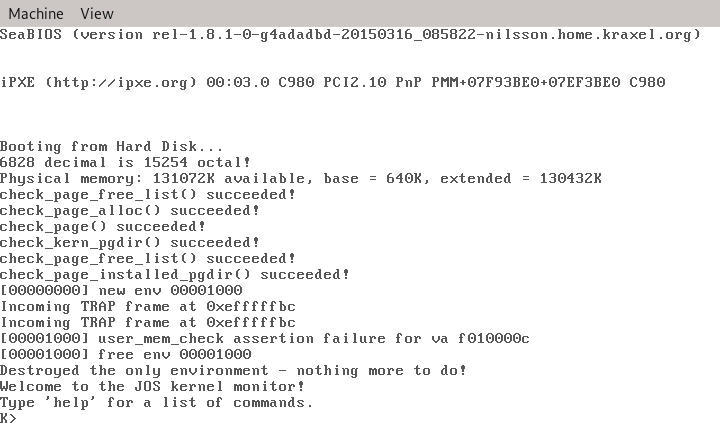
\includegraphics[width=0.9\linewidth]{lab1/exercise10_1.png}
    \caption{调用test\_backtrace(5)前的栈寄存器信息}
    \label{fig:exercise10_1}
\end{figure}
\par 在调用过程中,首先call指令将i386\_init的返回地址压入栈中,此时esp变为0xf010ffdc,此时进入test\_backtrace(5)子程序。然后开始执行上述的5个指令:push \%ebp用于保存\%ebp寄存器的值,执行完成后\%esp变为0xf010ffd8;然后 mov \%esp, \%ebp 把\%ebp的值更新为\%esp的值,也就是0xf010ffd8;然后push \%ebt保护寄存器\%ebx的值,执行完成后esp变为0xf010ffd4;最后sub \$0x14, \%esp将\%esp减去0x14,\%esp变为0xf010ffc0,这是用于分配空间存储临时变量。因此,在执行完上述指令后,\%esp和\%ebp分别变为0xf010ffc0和0xf010ffd8。而这就是test\_backtrace(5)执行时栈寄存器的变化范围。由于递归调用,像这样的变化还需要执行test\_backtrace(4)\textasciitilde test\_backtrace(0) 5次。
\par 也就是说每次递归调用压入32字节,也就是8个32位字。在调用到test\_backtrace(0)时,\%esp将为0xf010ff20而\%ebp将为0xf010ff38。实际的调试过程也验证了这一点,如图\ref{fig:exercise10_2}所示。
\begin{figure}[htb]
    \centering
    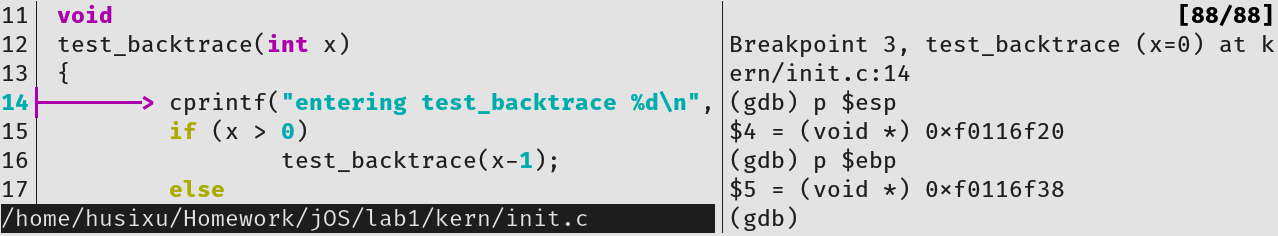
\includegraphics[width=0.9\linewidth]{lab1/exercise10_2.png}
    \caption{执行到test\_backtrace(0)时的栈寄存器值}
    \label{fig:exercise10_2}
\end{figure}
\FloatBarrier
\end{exerciseSolution}

\par 上述练习已经有足够多的信息以供实现一个stack backtrace程序了,将之称为mon\_backtrace(),其原型已经定义在kern/monitor.c中。除了实现之外,好需要将其hook到kernel monitor命令列表中,使其能够直接被用户调用。
\par backtrace函数应该显示一个如下的调用帧关系:
\inputCodeSetLanguage{bash}
\begin{lstlisting}[numbers=none]
Stack backtrace:
  ebp f0109e58  eip f0100a62  args 00000001 f0109e80 f0109e98 f0100ed2 00000031
  ebp f0109ed8  eip f01000d6  args 00000000 00000000 f0100058 f0109f28 00000061
  ...
\end{lstlisting}
\par 每一行都包含ebp, eip和args,也就是有关的寄存器以及参数。而第一行的Stack backtrace表明现在执行的是mon\_backtrace子程序。其后依次外推直到最外层。

\exercise{11}{
    \par 实现上述backtrace程序,并使用相同的格式进行输出。使用make grade进行验证。
}
\begin{exerciseSolution}{11}
    \par 根据程序调用时栈的关系来实现显示正在执行的程序的栈的信息,栈的结构如图\ref{fig:exercise11_1}所示。
    \par 可以看出,保存的\%ebp是连接当前栈帧和上一个(调用者的)栈帧的关键,它使各个栈帧通过类似于链表的结构连接起来。最终,在mon\_backtrace中填写的代码如下:
    \inputCodeSetLanguage{c}
    \begin{lstlisting}
int mon_backtrace(int argc, char **argv, struct Trapframe *tf) {
    uint32_t ebp, eip;
    cprintf("Stack backtrace:\n");
    for (ebp = read_ebp(); ebp != 0; ebp = *((uint32_t *)ebp)) {
        eip = *((uint32_t *)ebp + 1);
        cprintf("  ebp %08x  eip %08x  args %08x %08x %08x %08x %08x\n",
            ebp, eip, *((uint32_t *)ebp + 2),
            *((uint32_t *)ebp + 3), *((uint32_t *)ebp + 4),
            *((uint32_t *)ebp + 5), *((uint32_t *)ebp + 6));
    }
    return 0;
}
    \end{lstlisting}
    \begin{figure}[htb]
        \centering
        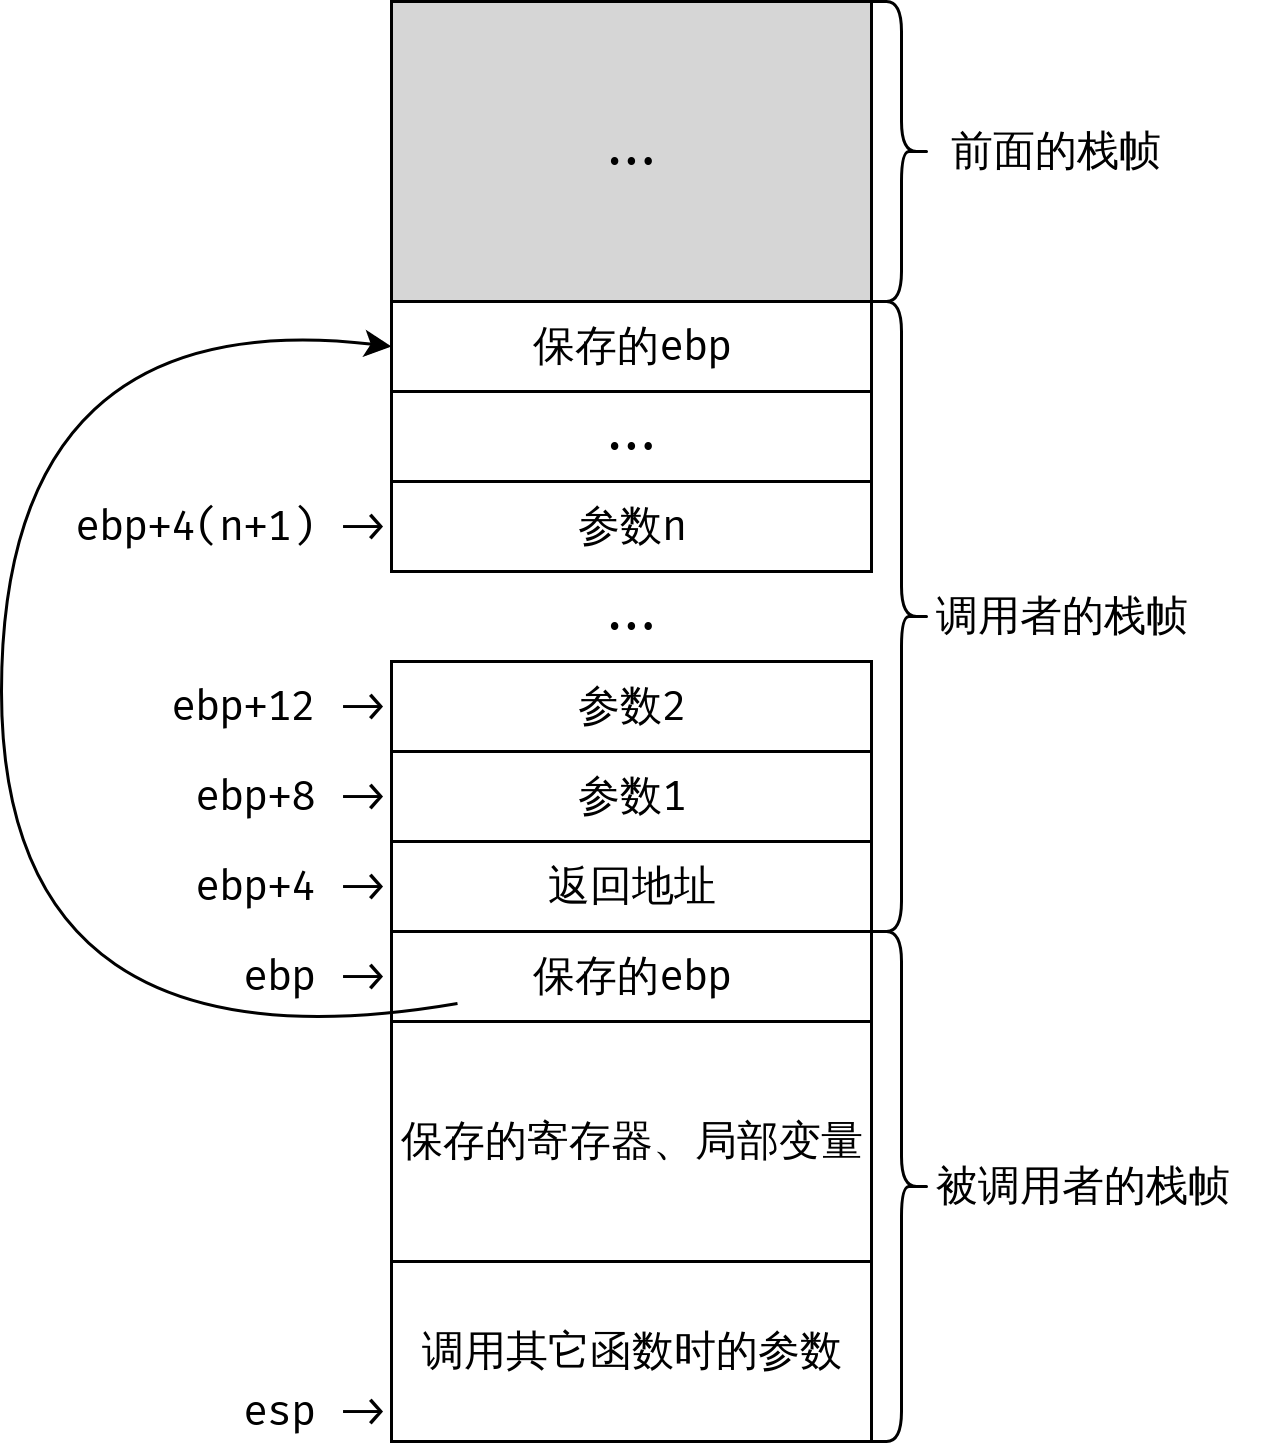
\includegraphics[width=0.4\linewidth]{lab1/exercise11_1.png}
        \caption{栈帧结构}
        \label{fig:exercise11_1}
    \end{figure}

    \par 使用make grade进行测试,结果如图\ref{fig:exercise11_2}所示。从结果中可以看出,backtrace count以及backtrace arguments已经通过测试,余下的backtrace arguments和backtrace lines需要在exercise 12中进一步补全。
    \begin{figure}[htb]
        \centering
        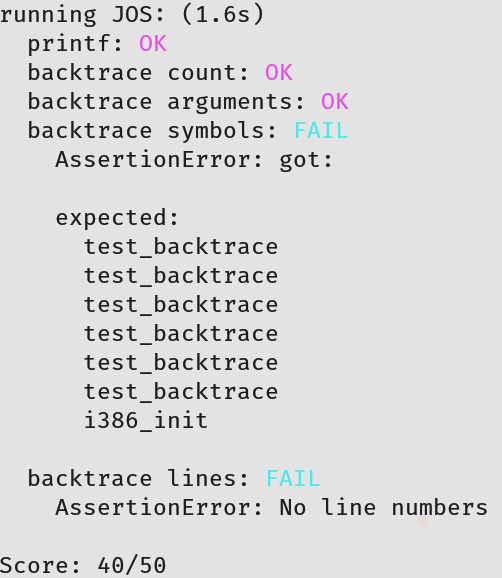
\includegraphics[width=0.4\linewidth]{lab1/exercise11_2.png}
        \caption{测试结果}
        \label{fig:exercise11_2}
    \end{figure}

    \FloatBarrier
\end{exerciseSolution}

\begin{exerciseEnv}{12}

    \par 继续修改backtrace函数,令其对于每个eip能显示函数名,源文件以及对应的行数。
    \par 在debuginfo\_eip中,\_\_STAB\_* 是从哪来的?这个问题的答案很长,可能需要以下操作来帮助找到答案:
    \begin{itemize}
        \item 看看 kern/kernel.ld中有哪些\_\_STAB\_*
        \item 运行 objdump -h obj/kern/kernel
        \item 运行 objdump -G obj/kern/kernel
        \item 运行 gcc -pipe -nostdinc -O2 -fno-builtin -I. -MD -Wall -Wno-format -DJOS\_KERNEL -gstabs -c -S kern/init.c,然后查看init.s
        \item 看看bootloader是否将符号表作为内核的一部分加载到了内存中。
    \end{itemize}
    \par 继续完成debuginfo\_eip的实现,通过调用stab\_binsearch来查找地址对应的行数。
    \par 在kernel monitor中添加backtrace命令,并扩展mon\_backtrace函数,令其调用debuginfo\_eip然后对于每一个栈帧打印如下格式的一行:
    \inputCodeSetLanguage{bash}

    \begin{lstlisting}[numbers=none,framexleftmargin=0mm,xleftmargin=0mm]
Stack backtrace:
  ebp f010ff78  eip f01008ae  args 00000001 f010ff8c 00000000 f0110580 00000000
         kern/monitor.c:143: monitor+106
  ebp f010ffd8  eip f0100193  args 00000000 00001aac 00000660 00000000 00000000
         kern/init.c:49: i386\_init+59
  ebp f010fff8  eip f010003d  args 00000000 00000000 0000ffff 10cf9a00 0000ffff
         kern/entry.S:70: <unknown>+0
    \end{lstlisting}
    \par 每一行都给出了文件名以及行号,紧跟着的是函数名以及eip相对于这个函数第一条指令的偏移。
\end{exerciseEnv}

\begin{exerciseSolution}{12}
    \par stab表是用于存储源文件以及编译后文件对应关系的一张表。使用objdump -G obj/kern/kernel命令,查看stab表中的内容,其输出如图\ref{fig:exercise12_1}所示。
    \begin{figure}[htb]
        \centering
        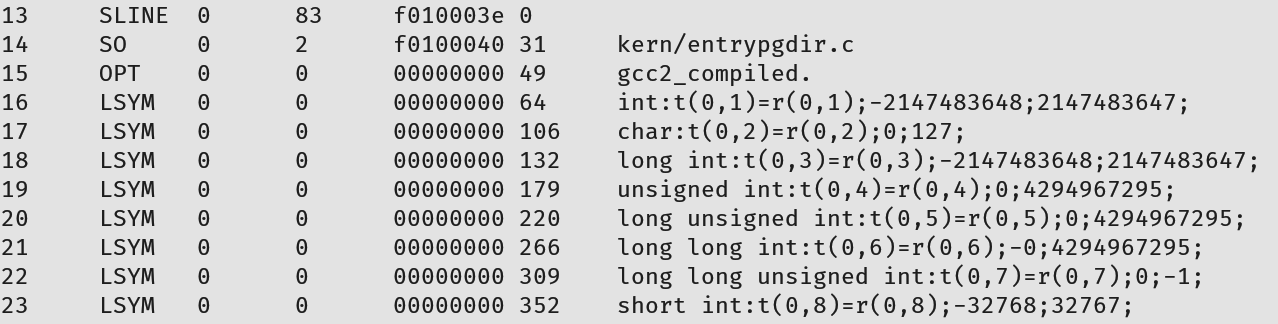
\includegraphics[width=0.9\linewidth]{lab1/exercise12_1.png}
        \caption{stab表部分内容}
        \label{fig:exercise12_1}
    \end{figure}
    \par 图中,前五列对应的就是stab,第7列是stabstr,分别对应着kdebug.c中的\_\_STAB\_BEGIN\_\_以及\_\_STABSTR\_BEGIN\_\_。
    \par 通过stab\_binsearch对于stab进行检索。通过注释可以知道stab\_binsearch接受4个参数:
    \begin{itemize}
        \item const struct Stab *stabs:stab表的起始位置。
        \item int *region\_left:查找下界。
        \item int *region\_right:查找上界。
        \item int type:查找的表项类型,对应图\ref{fig:exercise12_1}的第二列
        \item uintptr\_t addr要查找的值,对应图\ref{fig:exercise12_1}的第五列。
    \end{itemize}
    \par 通过这个函数对于stab表进行查找,可知在debuginfo\_eip中需要补全的部分为:
    \inputCodeSetLanguage{c}
    \begin{lstlisting}
stab_binsearch(stabs, &lline, &rline, N_SLINE, addr);
info->eip_line = lline > rline ? -1 : stabs[rline].n_desc;
    \end{lstlisting}

    \par 将debuginfo\_eip补全以后,需要对于kern/monitor.c中的mon\_backtrace进行扩展,使其调用这一函数以获得相应的调试信息。扩展后的mon\_backtrace如下:
    \begin{lstlisting}
int mon_backtrace(int argc, char **argv, struct Trapframe *tf) {
    uint32_t ebp, eip;
    struct Eipdebuginfo info;
    cprintf("Stack backtrace:\n");
    for (ebp = read_ebp(); ebp != 0; ebp = *((uint32_t *)ebp)) {
        eip = *((uint32_t *)ebp + 1);
        debuginfo_eip(eip, &info);
        cprintf("  ebp %08x  eip %08x  args %08x %08x %08x %08x %08x\n      %s:%d: %.*s+%d\n",
            ebp, eip,
            *((uint32_t *)ebp + 2), *((uint32_t *)ebp + 3), *((uint32_t *)ebp + 4),
            *((uint32_t *)ebp + 5), *((uint32_t *)ebp + 6),
            info.eip_file, info.eip_line, info.eip_fn_namelen,
            info.eip_fn_name, eip - info.eip_fn_addr);
    }
    return 0;
}
    \end{lstlisting}
    \par 然后重新编译,运行make grade的结果如图\ref{fig:exercise12_2}所示,可以看到已经通过全部的测试。
    \begin{figure}[htb]
        \centering
        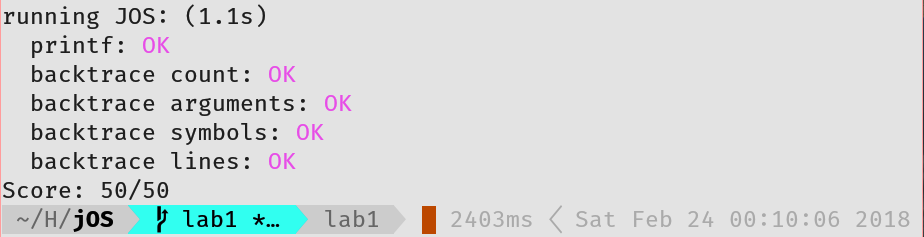
\includegraphics[width=0.9\linewidth]{lab1/exercise12_2.png}
        \caption{重新编译后运行make grade结果}
        \label{fig:exercise12_2}
    \end{figure}
    \par 最后,需要将backtrace命令整合进入终端中,这时只需将kern/monitor.c中的commands更改为如下几行即可。
    \begin{lstlisting}
static struct Command commands[] = {
    { "help", "Display this list of commands", mon_help },
    { "kerninfo", "Display information about the kernel", mon_kerninfo },
    { "backtrace", "Display information about function call frames", mon_kerninfo },
};
    \end{lstlisting}
    \par 更改后重新编译并进入qemu进行测试,可以看到,输入help后能够显示backtrace命令,并且输入backtrace后能够正确的输出结果了,如图\ref{fig:exercise12_3}所示。
    \begin{figure}[htb]
        \centering
        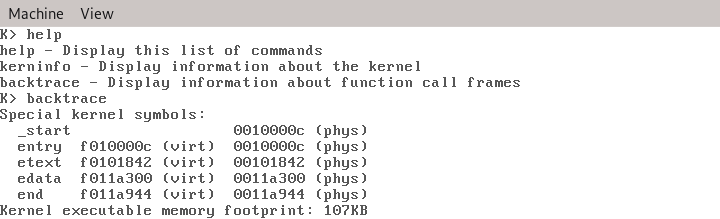
\includegraphics[width=0.8\linewidth]{lab1/exercise12_3.png}
        \caption{将backtrace整合到终端中}
        \label{fig:exercise12_3}
    \end{figure}
    \FloatBarrier
\end{exerciseSolution}


